\documentclass{tudelft-report.cls}

%% Set up the bibliography
\usepackage[sorting=none, citestyle=ieee, backend=biber]{biblatex}
\addbibresource{report.bib}
\usepackage{hyperref}
\usepackage{gensymb}
\usepackage{tabulary}
\usepackage{listings}
\usepackage{minted}
\usemintedstyle{pastie}
\usepackage{bm}
\usepackage{lipsum}             
\usepackage{xargs}              
\usepackage[colorinlistoftodos]{todonotes}
\usepackage{lscape}
\usepackage{graphicx}
\usepackage[british]{babel}
\usepackage{csquotes}
\usepackage{graphics}
\usepackage{multicol}
\usepackage{parskip}
\usepackage{adjustbox}
\usepackage{longtable}
\usepackage{lipsum}% this is dummy code
%\usepackage{pgfgantt}
\usepackage{wrapfig}
\usepackage{graphicx}
\usepackage{afterpage}
\usepackage{multirow}
\usepackage{colortbl}
\usepackage{hhline}
\usepackage[paper=A4,pagesize]{typearea}
\geometry{a4paper,hscale=0.8,vscale=0.75}
\KOMAoptions{DIV=15}

\sisetup{
     detect-all,
    exponent-mode = threshold,
    exponent-thresholds = -3:5,
    per-mode = symbol,
    round-mode = none,  % maybe change to "figures"
    round-precision = 3,
    round-pad = false, % whether their are extra trailing 0s
    output-decimal-marker = {.},
    group-digits = integer,
    output-exponent-marker = e,
    tight-spacing = false,
    list-units = single,
    product-units = single,
    range-units = single,
}

%% Additional packages and commands
\usepackage{parskip}
\setlist{itemsep=-2pt} % Reducing white space in lists slightly
\renewcommand{\deg}{\si{\degree}\xspace} % Use \deg easily, everywhere
\newcommand{\bfemph}[1]{\textbf{\emph{#1}}} % Bold and italic

%% ----------------------------------------------------------------------
%%    Begin of document + Frontmatter (Roman page numbering)
%% ----------------------------------------------------------------------

\begin{document}

\frontmatter

%% Define the main parameters
\title{Transwing eVTOL Project Plan}
%\subtitle{A Catchy Optional Subtitle \\ that Grabs the Attention}
\author{Project Group 1}

\subject{AE3200: Design Synthesis Excersise} % Cover only
\affiliation{Delft University of Technology} % Cover only
\coverimage{figures/cover.jpg} % Aspect ratio of 2:3 (portrait) recommended
\definecolor{title}{HTML}{4884d6} % Color for cover title

%\makecover

% \begin{titlepage}

% \begin{center}

% %% Print the title
% {\makeatletter
% \largetitlestyle\fontsize{45}{45}\selectfont\@title
% \makeatother}

% %% Print the subtitle
% {\makeatletter
% \ifdefvoid{\@subtitle}{}{\bigskip\titlestyle\fontsize{20}{20}\selectfont\@subtitle}
% \makeatother}

% \bigskip
% \bigskip

% by

% \bigskip
% \bigskip

% %% Print the name of the author
% {\makeatletter
% \largetitlestyle\fontsize{25}{25}\selectfont\@author
% \makeatother}

% \bigskip
% \bigskip

% %% Print table with names and student numbers
% \setlength\extrarowheight{2pt}
% \begin{tabular}{lc}
%     Student Name & Student Number \\\midrule
%     First Surname & 1234567 \\
% \end{tabular}

% \vfill

% %% Print some more information at the bottom
% \begin{tabular}{ll}
%     Tutors: &  I. Surname\\
%     Coaches: & I. Surname \\
%     Teaching Assistant: & I. Surname \\
%     Project Duration: & April, 2024 - June, 2024 \\
%     Faculty: & Faculty of Aerospace Engineering, Delft
% \end{tabular}

% \bigskip
% \bigskip

% %% Add a source and description for the cover and optional attribution for the template
% \begin{tabular}{p{15mm}p{10cm}}
%     Cover: & Canadarm 2 Robotic Arm Grapples SpaceX Dragon by NASA under CC BY-NC 2.0 (Modified) \\
%     % Feel free to remove the following attribution, it is not required - still appreciated :-)
%     Style: & TU Delft Report Style
% \end{tabular}

% \end{center}

% %% Insert the TU Delft logo at the bottom of the page
% \begin{tikzpicture}[remember picture, overlay]
%     \node[above=10mm] at (current page.south) {%
%         
\includegraphics{figures/logo-black}
%     };
% \end{tikzpicture}

% \end{titlepage}
\begin{titlepage}

\begin{center}

%% Print the title
{\makeatletter
\largetitlestyle\fontsize{45}{45}\selectfont\@title
\makeatother}

%% Print the subtitle
{\makeatletter
\ifdefvoid{\@subtitle}{}{\bigskip\titlestyle\fontsize{20}{20}\selectfont\@subtitle}
\makeatother}

\bigskip
\bigskip

by

\bigskip
\bigskip

%% Print the name of the author
{\makeatletter
\largetitlestyle\fontsize{25}{25}\selectfont\@author
\makeatother}

\bigskip
\bigskip

%% Print table with names and student numbers
\setlength\extrarowheight{2pt}
\begin{tabular}{lc}
    Student Name              & Student Number \\\midrule
    Alessandro Tesse          & 5471990 \\
    Brădut-Constantin Stanciu & 5534682 \\
    Ezra Cerpac               & 5259347 \\
    Gregorio Boccaccini       & 5484650 \\
    Koen Pijnacker            & 5559138 \\
    Philip Groenemeijer       & 5335574 \\
    Salman Mughal             & 5478847 \\
    Stefano Kok               & 4656091 \\
    Tim Guezen                & 5565448 \\
    Zoli Túri                 & 5213762 \\
\end{tabular}

\vfill

%% Print some more information at the bottom
\begin{tabular}{ll}
    Tutors: &  F. Scarano, F. Schrijer \\
    Coaches: & M. Moradi, T. de Ponti \\
    Teaching Assistant: & A. F. Khalil \\
    Project Duration: & April - June, 2024 \\
    Faculty: & Faculty of Aerospace Engineering, Delft
\end{tabular}

\bigskip
\bigskip

%% Add a source and description for the cover and optional attribution for the template
%\begin{tabular}{p{15mm}p{10cm}}
%    Cover: & Canadarm 2 Robotic Arm Grapples SpaceX Dragon by NASA under CC BY-NC 2.0 (Modified) \\
%    % Feel free to remove the following attribution, it is not required - still appreciated :-)
%%    Style: & TU Delft Report Style
%\end{tabular}

\end{center}

%% Insert the TU Delft logo at the bottom of the page
\begin{tikzpicture}[remember picture, overlay]
    \node[above=10mm] at (current page.south) {%
        
\includegraphics{figures/logo-black}
    };
\end{tikzpicture}

\end{titlepage}

%\chapter*{Preface}
\addcontentsline{toc}{chapter}{Preface}

\emph{A preface...}

\begin{flushright}
{\makeatletter\itshape
    \@author \\
    Delft, \monthname{} \the\year{}
\makeatother}
\end{flushright}

%\chapter*{Summary}
\addcontentsline{toc}{chapter}{Summary}



\tableofcontents
%\listoffigures
%\listoftables

%\chapter*{Nomenclature}
\addcontentsline{toc}{chapter}{Nomenclature}

\emph{If a nomenclature is required, a simple template can be found below for convenience. Feel free to use, adapt or completely remove.}

\section*{Abbreviations}

\begin{longtable}{p{2.5cm}p{8cm}}
    \toprule
    Abbreviation & Definition \\
    \midrule\endhead % Add abbreviations alphabetically here:
    ISA & International Standard Atmosphere \\
    CE & Chief Engineer \\
    \bottomrule
\end{longtable}

\section*{Symbols}

\begin{longtable}{p{2.5cm}p{8cm}p{2.5cm}}
    \toprule
    Symbol & Definition & Unit \\
    \midrule\endhead % Add Latin symbols alphabetically here:
    $V$ & Velocity & [m/s] \\
    ... \\
    \midrule % Add Greek symbols alphabetically here:
    $\rho$ & Density & [kg/m$^3$] \\
    ... \\
    \bottomrule
\end{longtable}


%% ----------------------------------------------------------------------
%%    Mainmatter (Arabic page numbering)
%% ----------------------------------------------------------------------

\mainmatter

% \input{mainmatter/introduction}

% \let\oldcleardoublepage\cleardoublepage
% \let\oldclearpage\clearpage
% \renewcommand{\cleardoublepage}{}
% \renewcommand{\clearpage}{}


%% From the deliverables description:
% General Summary
% User Requirements  
% Description of the entire system (the Global Picture)  
% Technical Design Development Organisational Breakdown Structure (organogram with the   responsibilities of the various group members) 
% Work Flow Diagram (WFD)
% Work Breakdown Structure (WBS)  
% Schedule (Gantt chart)
% Project rules 
% Organisational risk assessment 
% Project Approach with respect to sustainable development (not technical!)  
% References
% Appendices


% \input{mainmatter/uncatagorised}
\chapter{General Summary}
\label{ch:General_Summary}
This chapter will give a broad overview of what the "Transwing eVTOL" project consists of.
In \cref{sec:description-of-entire-system} more context about the project will be given, from which the Mission Need Statement (MNS) and the Project Objective Statement (POS) will flow.
\Cref{sec:customer-requirements} will lastly state the top-level requirements defined by the customer interested in the development and establishment of this technology.

\section{Description of Entire System}
\label{sec:description-of-entire-system}
This project aims to fill a gap in the aviation market, namely Inter-Urban Air Mobility (I-UAM).
UAM is an emerging branch of Air Mobility rapidly gaining traction in both the industry and scientific community \cite{UAM-Overview}.
It entails the use of small, highly automated aircraft for passenger or cargo transportation in urban areas, similar to cars used today.
Vertical Take-Off and Landing (VTOL) vehicles are preferred when constraints are put on the maximum ground footprint of the aircraft.
The currently certified VTOL models for UAM mostly consist of wingless rotorcrafts.
However, wings offer many advantages when it comes to efficient (cruise) flight over longer distances; to achieve I-UAM, and thereby facilitate travel between cities, wings offer a big advantage in terms of performance and design.
To design a low ground footprint VTOL, a transwing option is proposed.
Finally, the vehicle should be electric to reduce emissions, and noise pollution in urban areas and therefore increase product sustainability.
The above considerations result in the following Mission Need Statement (MNS) and Project Objective Statement (POS).

\paragraph{MNS:}“\textit{Achieve Sustainable Inter-Urban Air Mobility with a low ground footprint vehicle.}”
\vspace{-5mm}
\paragraph{POS:}“\textit{Design a low ground footprint, sustainable, urban transwing electric Vertical Take-Off and Landing vehicle within production costs of \num{2000}kEUR, by 10 students in 10 weeks time.}”



\section{Requirements}\label{sec:customer-requirements}
The first set of requirements given can be divided into the following main categories: performance, safety, customer, cost \& sustainability.
Below, the top-level system requirements are listed in the words of the customer. These initial requirements will be further elaborated upon in the first phases of the design. 

% \begin{table}[H]
% \centering
% \caption{Vehicle Requirements Specification}
% \label{tab:vehicle_requirements}
% \begin{tabular}{|l|p{10cm}|}
% \hline
% \textbf{ID} & \textbf{Requirement} \\ \hline
% \multicolumn{2}{|c|}{\textbf{Performance}} \\ \hline
% REQ-001 & Maximum payload weight of 400 kg \\ \hline
% REQ-002 & Indicative maximum size is 8 x 4 x 1 m\textsuperscript{3} on the ground \\ \hline
% REQ-003 & Cruise speed of 200 km/h \\ \hline
% REQ-004 & Compliance with European noise emission regulations \\ \hline
% REQ-005 & Electric power autonomy for 100 km + reserve \\ \hline
% REQ-006 & Lifetime of the vehicle should be greater than 10 years \\ \hline
% \multicolumn{2}{|c|}{\textbf{Safety}} \\ \hline
% REQ-007 & Adoption of an autopilot and proximity sensors \\ \hline
% REQ-008 & Operational at 5 m distance from people and 3 m from any object in densely populated areas \\ \hline
% REQ-009 & Compliance with aero-acoustic regulations for emissions over urban areas, and maximum cabin noise of 60 dBA \\ \hline
% \multicolumn{2}{|c|}{\textbf{Customer Requirements}} \\ \hline
% REQ-010 & Capability for overnight flight \\ \hline
% REQ-011 & Flight in windy conditions, up to 8 Beaufort, with or without rain \\ \hline
% REQ-012 & Redundant propulsive system that can fly with 75\% of the system actively working \\ \hline
% \multicolumn{2}{|c|}{\textbf{Cost and Sustainability}} \\ \hline
% REQ-013 & Final product cost not exceeding 2000 kEUR \\ \hline
% REQ-014 & Main structure should be reusable for at least 10 years and then easily recyclable \\ \hline
% \end{tabular}
% \end{table}


\begin{table}[H]
\centering
\caption{Vehicle Requirements Specification}
\label{tab:vehicle_requirements}
\renewcommand{\arraystretch}{0.85}
\begin{tabularx}{\linewidth}{|l|>{\centering\arraybackslash}X|}
\hline
\textbf{ID} & \textbf{Performance Requirements} \\ \hline
REQ-PERF-001 & Maximum payload weight of 400 kg \\ \hline
REQ-PERF-002 & Indicative maximum size is 8 x 4 x 1 m\(^3\) on the ground \\ \hline
REQ-PERF-003 & Cruise speed of 200 km/h \\ \hline
REQ-PERF-004 & Compliance with European noise emission regulations \\ \hline
REQ-PERF-005 & Electric power autonomy for 100 km + reserve \\ \hline
REQ-PERF-006 & Lifetime of the vehicle should be greater than 10 years \\ \hline
\textbf{ID} & \textbf{Safety Requirements} \\ \hline
REQ-SAF-001 & Adoption of an autopilot and proximity sensors \\ \hline
REQ-SAF-002 & Operational at 5 m distance from people and 3 m from any object in populated areas \\ \hline
REQ-SAF-003 & Maximum cabin noise of 60 dBA \\ \hline
\textbf{ID} & \textbf{Customer Requirements} \\ \hline
REQ-CUST-001 & Capability for overnight flight \\ \hline
REQ-CUST-002 & Flight in windy conditions, up to 8 Beaufort, with or without rain \\ \hline
REQ-CUST-003 & Redundant propulsive system that can fly with 75\% of the system actively working \\ \hline
\textbf{ID} & \textbf{Cost and Sustainability Requirements} \\ \hline
REQ-COST-001 & Final product cost not exceeding 2000 kEUR \\ \hline
REQ-SUST-001 & Main structure should be reusable for at least 10 years and then easily recyclable \\ \hline
\end{tabularx}
\end{table}


\chapter{Technical Design Development}\label{ch:techdesdev}


\section{Organisational Breakdown Structure}\label{sec:orgbreakdown}
A clear division of roles and responsibilities is of paramount importance for a functional working environment, hence this chapter establishes all organisational and technical roles each member of the team has. This will be illustrated by an organogram in \cref{fig:orgbreakdownstruc}, and the responsibilities of each role are defined in \cref{sec:org-roles}, as this will keep the organogram as organised and concise as possible. Moreover, the initials of each team member can be seen in each role, clarifying and simplifying the organogram.

\begin{figure}[ht]
    \centering
    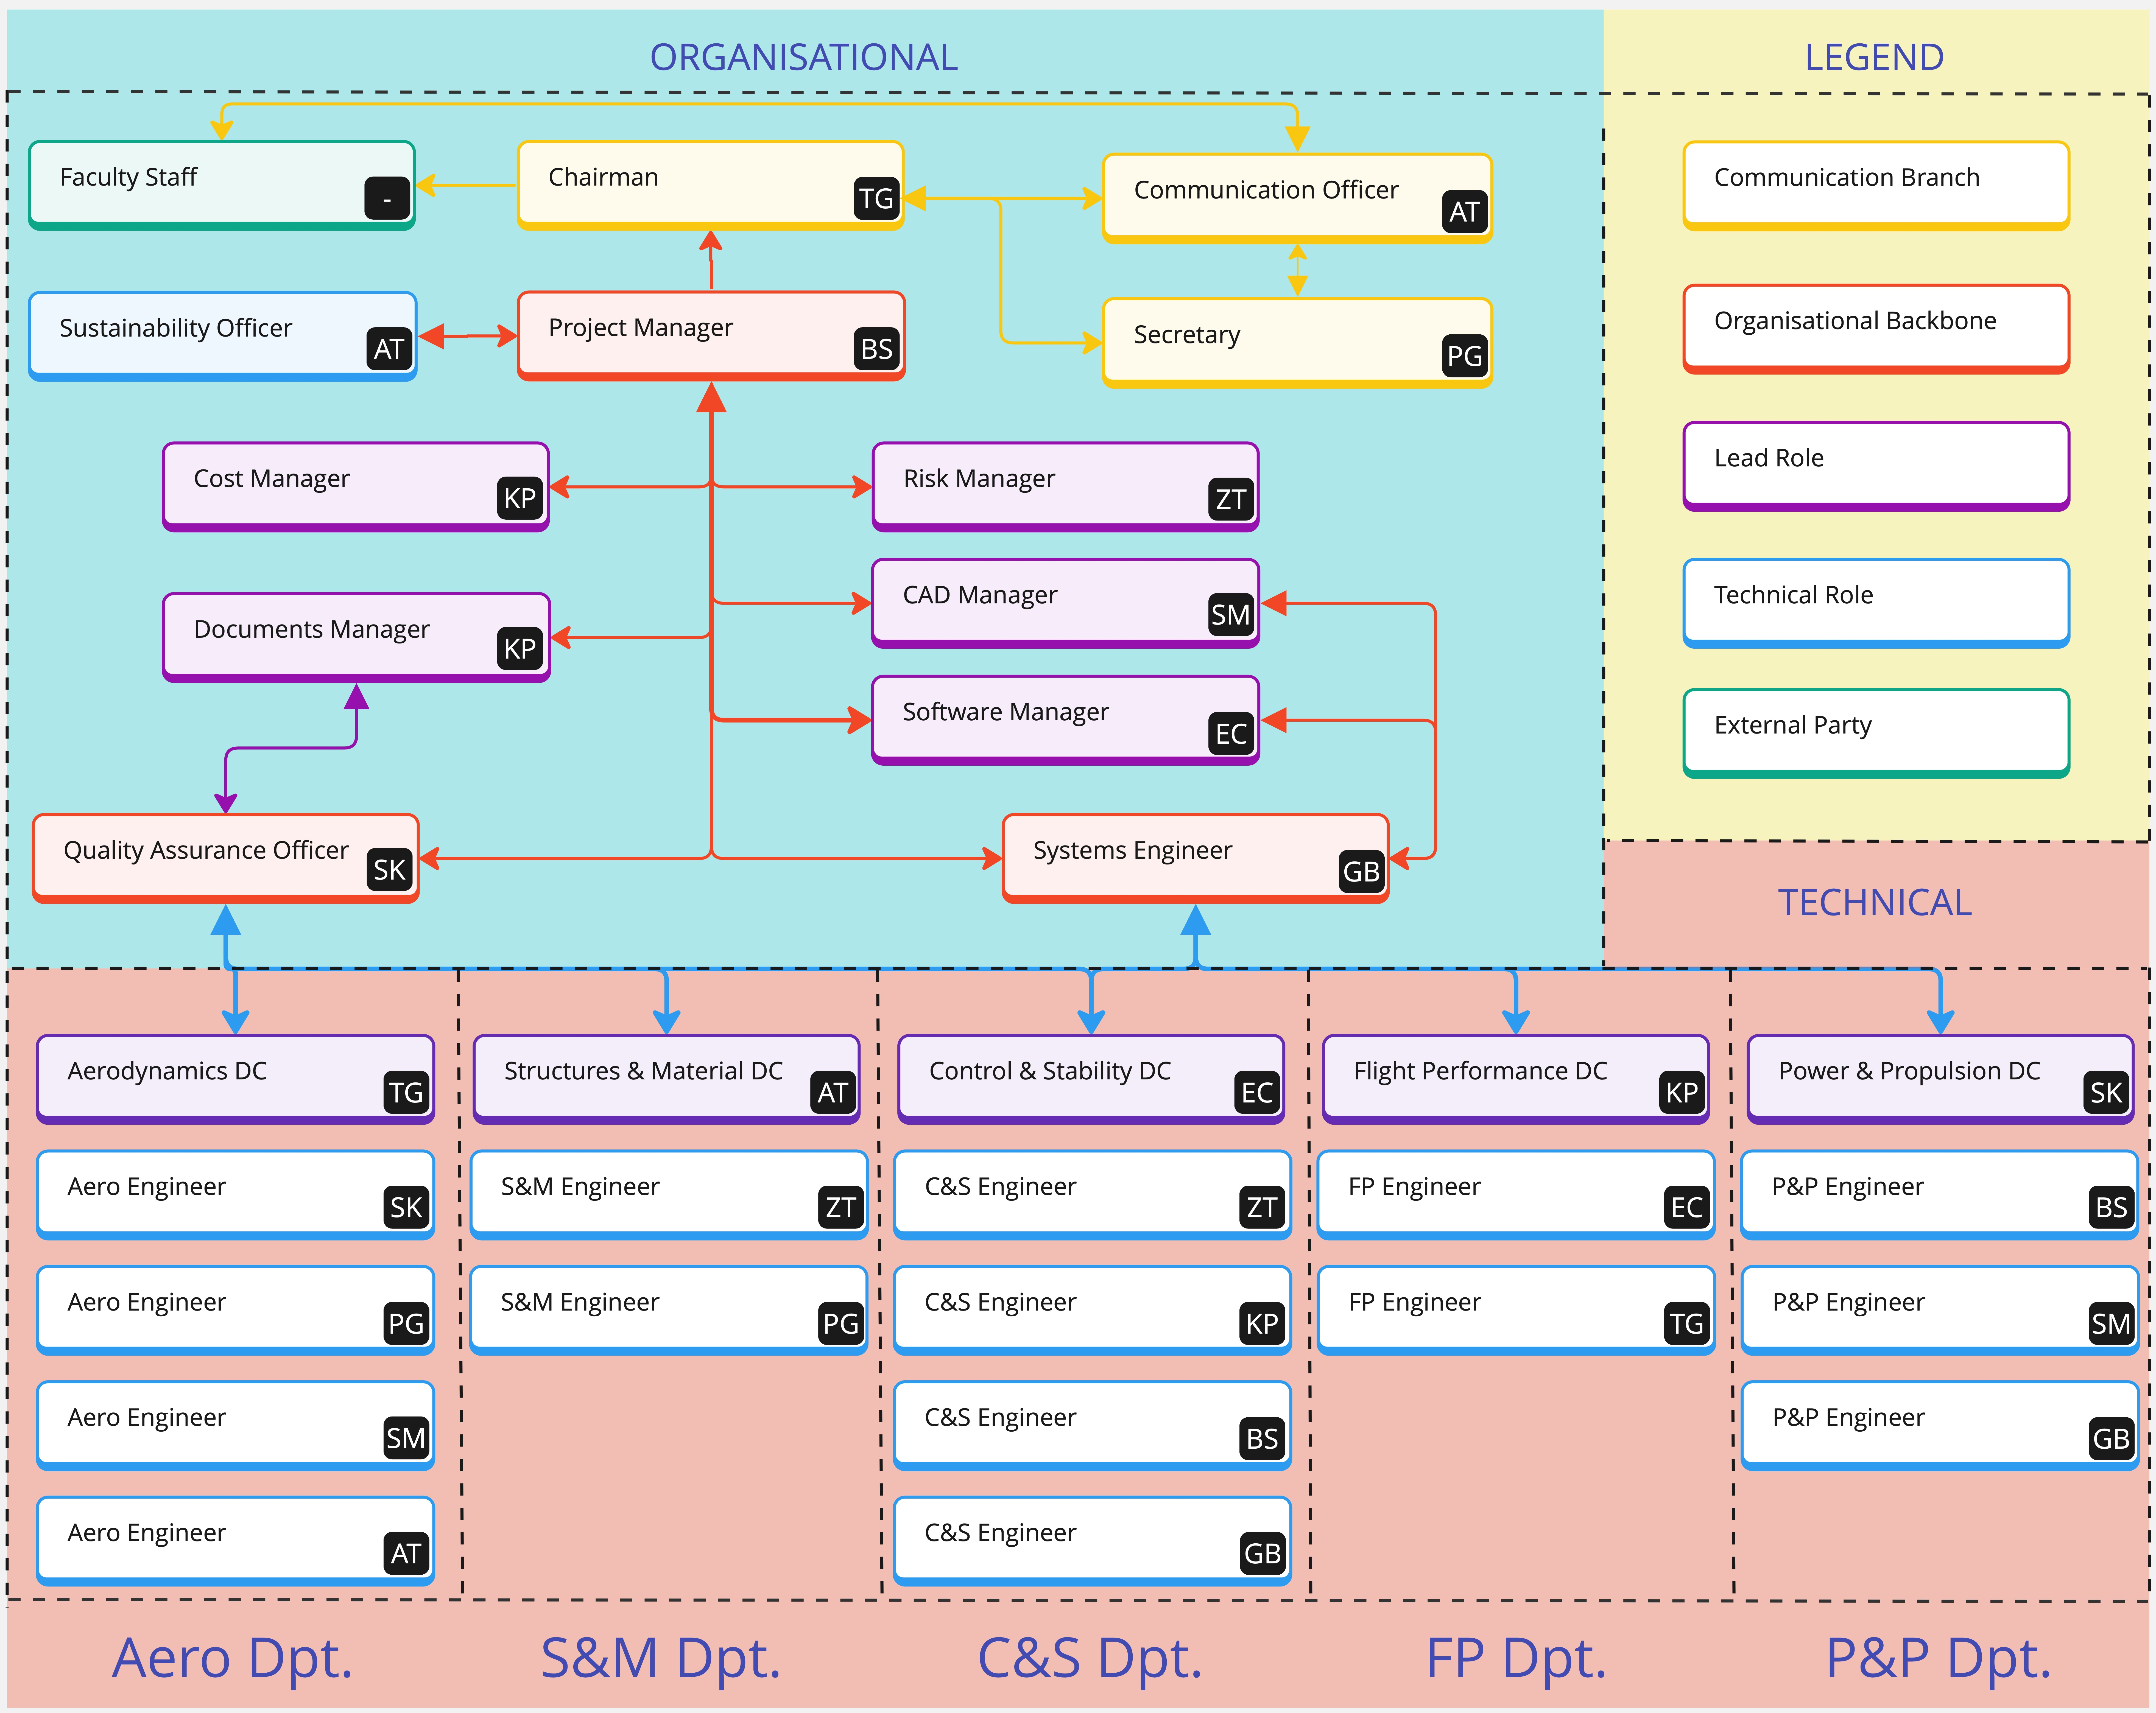
\includegraphics[width=\linewidth]{figures/Copy OBS.jpg}
    \caption{Organisational Breakdown Structure, the abbreviations of the members of the team are specified in .}
    \label{fig:orgbreakdownstruc}
\end{figure}


\subsection{Organisational Roles}\label{sec:org-roles}
The assigned responsibilities for all the organisational roles presented in \cref{fig:orgbreakdownstruc} are specified and elaborated on below:
\begin{itemize}
    \item \textbf{Project Manager (PM)}: The PM coordinates the team, manages resources, and ensures the project meets deadlines, and budgets and regulates proper sharing of information with the outside~\cite{dsePMSESlides1}.
    The responsibilities of the PM can be broken down into:
    \begin{itemize}
        \item \textit{The PM shall define the organisation and procedures of the project, along with ensuring sensible results, budget and resource allocation.}
        \item \textit{The PM shall closely follow and supervise the development of the Gantt Chart and the project schedule.}
        \item \textit{The PM shall constantly collect information on project status to be shared with the interested parties, define and take corrective/adaptive actions, and officially close out the project.}
    \end{itemize}
    \item \textbf{Chairman}: The Chairman, is the main communication link with the external parties, as can be deduced from \cref{fig:orgbreakdownstruc}.
    Furthermore, it oversees and controls the communication branch in its entirety, ensuring clear and effective communication between all the team members.
    The responsibilities of the Chairman can be broken down into:
    \begin{itemize}
        \item \textit{The Chairman shall lead the customer and staff meetings, by directing the discussion according to the meeting.}
        \item \textit{The Chairman shall be responsible for smooth communication with the secretary and communication officer.}
    \end{itemize}
    \item \textbf{Secretary}: The Secretary shall maintain and organise the various tasks, implement procedures and carry out administrative duties~\cite{SysEngrespons}.
    The responsibilities of the Secretary can be broken down into:
    \begin{itemize}
        \item \textit{The Secretary shall always be actively taking notes during meetings and global discussions within the group.}
        \item \textit{The Secretary is responsible for retrieving and preparing the agenda used as a reference for the meetings.}
    \end{itemize}
    \item \textbf{Communication Officer (CO)}: The CO is, besides the Chairman, the sole other member who is in direct communication with the faculty staff and other external parties, mainly through online communication (e.g. via e-mail).
    The responsibilities of the CO can be broken down into:
    \begin{itemize}
        \item \textit{The CO provides direct communication between the faculty staff and team, hence he is also responsible for a clear meeting schedule.}
        \item \textit{The CO shall ensure constant effective communication between all the team members.}
    \end{itemize}
    \item \textbf{Sustainability Officer (SO)}: The SO is responsible for guiding the team's effort towards an environmental, social and economical-conscious working approach~\cite{sustofficer}.
    As this is one of the greater areas of focus of the team, during the project;
    \item \textbf{Quality Assurance Officer (QAO)}: The QAO, alongside the SE, provides a clear connection between the organisational and technical sections of the organogram.
    Hence, the QAO has to be in clear and direct communication with the SE to ensure quality in the technical division.
    The responsibilities of the QAO can be broken down into:
    \begin{itemize}
        \item \textit{The QAO shall perform frequent, standardised and planned quality controls concerning content and progress of the project.}
        \item \textit{The QAO shall provide clear guidelines for writing and organisational and technical procedures.}
        \item \textit{The QAO shall provide the team with a clear plan to make the proofreading process as thorough and efficient as possible.}
    \end{itemize}
    \item \textbf{Systems Engineer (SE)}: The SE is responsible for the correct integration of complex systems, ensuring all components work together effectively to meet project requirements and objectives~\cite{SysEngrespons}.
    The responsibilities of the SE can be broken down into:
    \begin{itemize}
        \item \textit{The SE shall evaluate the current systems and identify and implement potential improvements.}
        \item \textit{The SE is in charge of the installation, configuration, improvement and monitoring of new systems, and monitors the implications that the systems usage has on the project.}
%        \item \textit{Coordination of affected departments and other interested parties, including the potential need for training.}  % should be removed I think, training is pretty for fetched for such a short project
%        \item \textit{Collaboration with team members, end users, clients, suppliers, and stakeholders with a focus on continuous improvement.}
        \item \textit{The SE shall integrate new systems within existing infrastructures, emphasising advantages, and minimising disruption.}
        \item \textit{The SE shall communicate the performance levels to management, often via presentations.}
    \end{itemize}
    \item \textbf{Documents Manager (DM)}: The DM shall make sure all the documents used within the project meet standards of quality, objectiveness, and accuracy, and that the industry and the scientific community officially recognise them.
    The responsibilities of the DM can be broken down into:
    \begin{itemize}
        \item \textit{The DM shall ensure that all the documents are of high scientific quality.}
        \item \textit{The DM shall also hold and maintain an archive with all the used documents, ensuring the team's process can be easily validated and traced back to official literature and references.}
        \item \textit{The DM shall also be responsible for the quality of the references used in the report.}
    \end{itemize}
    \item \textbf{Cost Manager (CM)}: The CM is responsible for monitoring and controlling project costs, developing and maintaining budget forecasts, identifying cost-saving opportunities, and ensuring the project remains within financial constraints while meeting its objectives and quality standards;
    \item \textbf{Risk Manager (RM)}: The RM is responsible for the identification, assessment, analysis, and handling of all possible risks, ensuring proper risk management over the entire team.
    \begin{itemize}
        \item \textit{The RM shall provide a methodology to identify, assess, analyse and handle (track, reduce or eliminate) all the possible risks.}
        \item \textit{The RM shall apply this methodology within each department to ensure proper risk management over the entire team.}
        \item \textit{The RM shall draft and further analyse the risk report.}
    \end{itemize}
    \item \textbf{Computer-Aided Design Manager (CADM)}: The CADM shall oversee the use of CAD software, and ensure that all drawings conform to the same standards and regulations.
    \begin{itemize}
        \item \textit{The CADM shall manage the CAD technicians, and ensure the accuracy and quality of all design drawings, as well as ensuring conformity to industry standards and regulations.}
        \item \textit{The CADM shall develop and implement CAD standards and workflows to optimize design processes and facilitate efficient project execution.}
        \item \textit{The CADM shall oversee the use of CAD software and hardware, and ensure that the CAD technicians are properly trained and equipped to use the software and hardware.}
    \end{itemize}
    \item \textbf{Software Manager (SM)}: the SM oversees the development, implementation, and maintenance of software systems
    \begin{itemize}
        \item \textit{The SM shall oversee the software systems' development, implementation, and maintenance.}
        \item \textit{The SM shall manage and fit the department-specific software writing within project timelines, and resources, whilst collaborating with project stakeholders to ensure the software meets all technical specifications and operational requirements.}
        \item \textit{The SM shall ensure that the software is developed according to the project's requirements and specifications.}
        \item \textit{The SM shall ensure that the software engineers are properly trained, and adhere to the project's software development standards, procedures and regulations.}
    \end{itemize}
\end{itemize}


\subsection{Technical Roles}\label{sec:technical-roles}
Before assigning the responsibilities of the technical roles shown in \cref{fig:orgbreakdownstruc}, it is important to specify the departments, which each have their own department chief (DC) directing their specialised engineers.
The team decided to divide the technical tasks into five departments: \textbf{Aerodynamics}, \textbf{Structures \& Materials}, \textbf{Control \& Stability}, \textbf{Flight Performance}, and \textbf{Power \& Propulsion}.
These are considered to be the main areas of focus during the project. 
The DCs are responsible for the coordination of their respective department, as can be deduced from \cref{fig:orgbreakdownstruc}.
Although focused towards coordination and management, the roles of the DCs will not clash with the SE, as the latter will mainly act as coordinator of all the DCs; ensuring correct implementation of the concept of Concurrent Engineering.
Moreover, the specified technical roles have not yet been established, as this will become more clear during the project.
However, the team did divide departments among the interests and expertise, to realise an efficient and healthy working environment.


\section{Project Logic Diagrams}\label{sec:projlogicdiag}
This section dives into the Logic Diagrams used to organise and control the project.
Tools like, the Work Flow Diagrams (WFD), Work Breakdown Structures (WBS), and Gantt Charts are crucial for completing a multi-disciplinary product development project successfully.
The Work Flow Diagram is presented and explained in \cref{sec:wfd}, the Work Breakdown Structure in \cref{sec:wbs}, and the Gantt Chart in \cref{sec:gantt-chart}.

\subsection{Work Flow Diagram}\label{sec:wfd}
To create a proper plan for the time frame and logic of the project, a Work Flow Diagram (WFD) is created.
It illustrates all the relevant deliverables of the project, as well as the necessary activities that are to be performed throughout the project.
A crucial aspect showcased with the help of the WFD is the relationship between different modules (activities or deliverables) of the project.
Thus, iterative activities can be showcased and predicted when organising the project.
Additionally, the WFD displays the responsible person for checking the progress of each of the main tasks.
Moreover, the total work effort required for each of the tasks, as well as the throughput time, are presented in the diagram.

To showcase the flow of the project more clearly, the project is split into six phases, and the flow between the phases and the main deliverables shall be presented in a reduced WFD present at the top of both pages, meant to showcase the project flow.
Afterwards, each of the six phases shall be presented in more detail by showcasing the inputs and outputs, and the constituent elements of every phase, as well as their interrelations.
All elements in the WFD are colour-coded, and referenced in the legend on both pages.

\afterpage{
    \KOMAoptions{paper=A3,paper=portrait,pagesize}
    \recalctypearea
    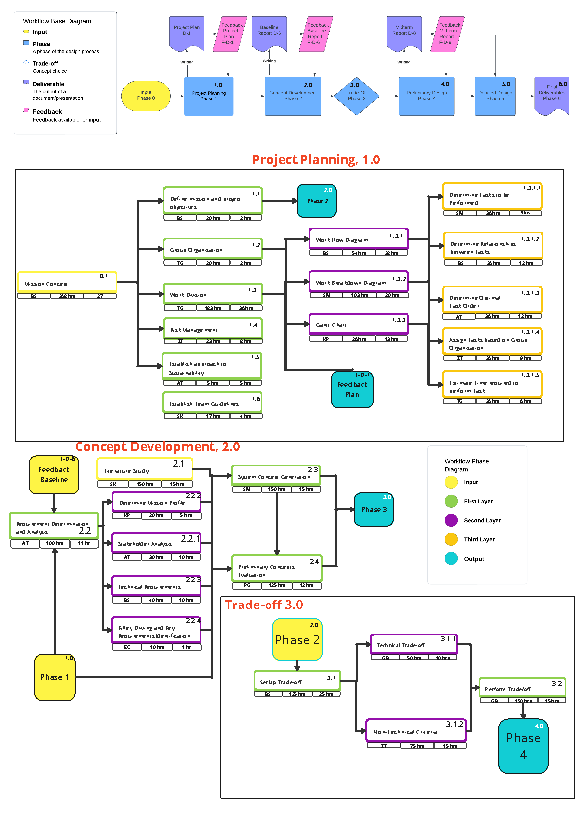
\includepdf{figures/workflowP1.pdf}
    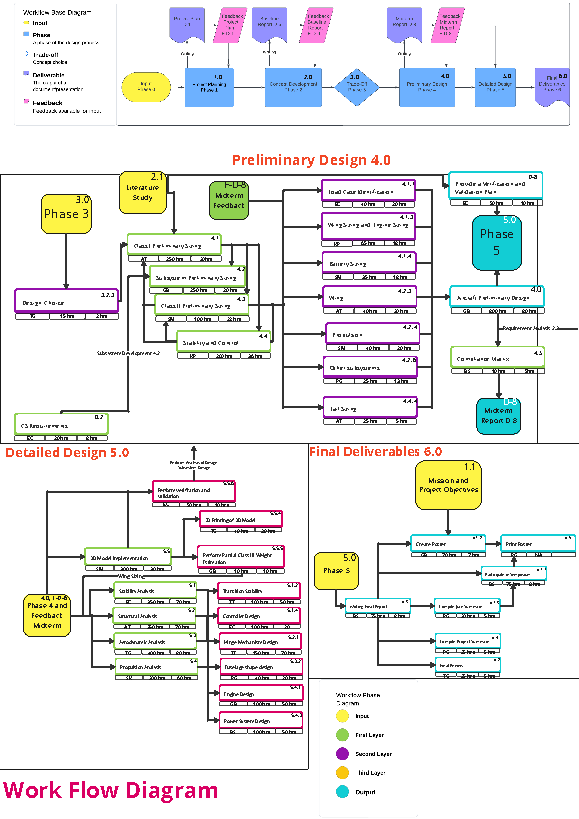
\includepdf{figures/workflowP2.pdf}
    %\clearpage
    \KOMAoptions{paper=A4,paper=portrait,pagesize}
    \recalctypearea
}

\subsection{Work Breakdown Structure}\label{sec:wbs}
From the WFD described in \cref{sec:wfd}, it is possible to derive the Work Breakdown Structure (WBS). This is an invaluable tool in project management, showcasing every phase and task that needs to be completed.
This diagram inherits the top layers of the project phases from the WFD and then breaks these layers into smaller tasks that can be visualized hierarchically. 
Like in the WFD, the responsible person, total time, and throughput time are displayed for every task in the WBS.
% Thanks to the WBS not only all the major processes of the project can be visualized, but it can also be used to create a Gantt chart, as will be explained later.

It is important to note that the sum of the hours in the Work Breakdown Structure does not equal 4000. This is because 300 man-hours are reserved for the PMSE lectures, the peer review of other reports, and the baseline and mid-term review meetings.
\afterpage{
    \KOMAoptions{paper=A3,paper=portrait,pagesize}
    \recalctypearea
    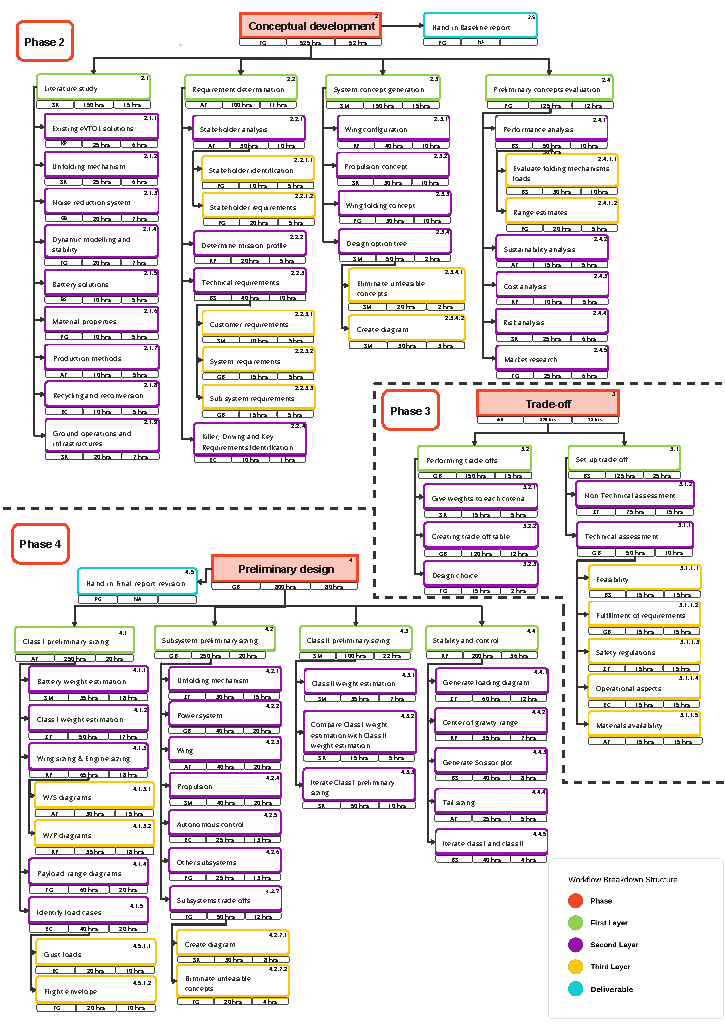
\includepdf{figures/breakdownP1.pdf}
    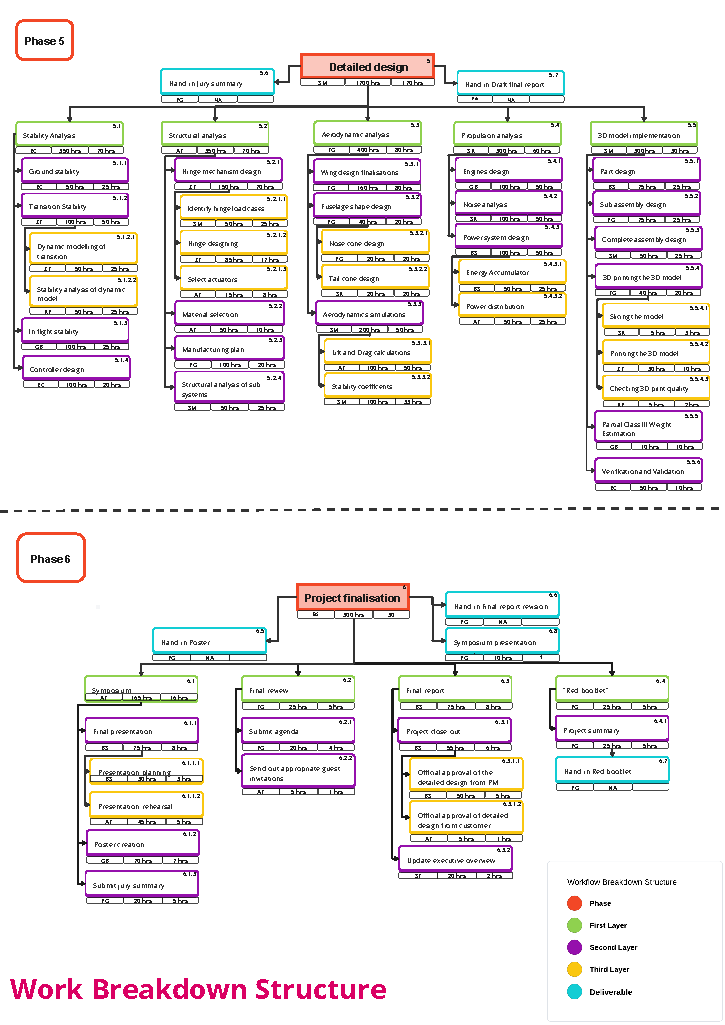
\includepdf{figures/breakdownP22.pdf}
    \KOMAoptions{paper=A4,paper=portrait,pagesize}
    \recalctypearea
}

\subsection{Gantt Chart}\label{sec:gantt-chart}
For the project planning a Gantt Chart was made. The Gantt Chart contains almost 200 tasks. Planning everything to the smallest detail is deemed unnecessary and counterproductive at this point in the design process. That is why only for the next project phase, the concept development phase, all tasks are planned in detail. For the subsequent phases of the project, the main structure is laid out. 

\afterpage{
    \KOMAoptions{paper=A3,paper=landscape,pagesize}
    \recalctypearea
    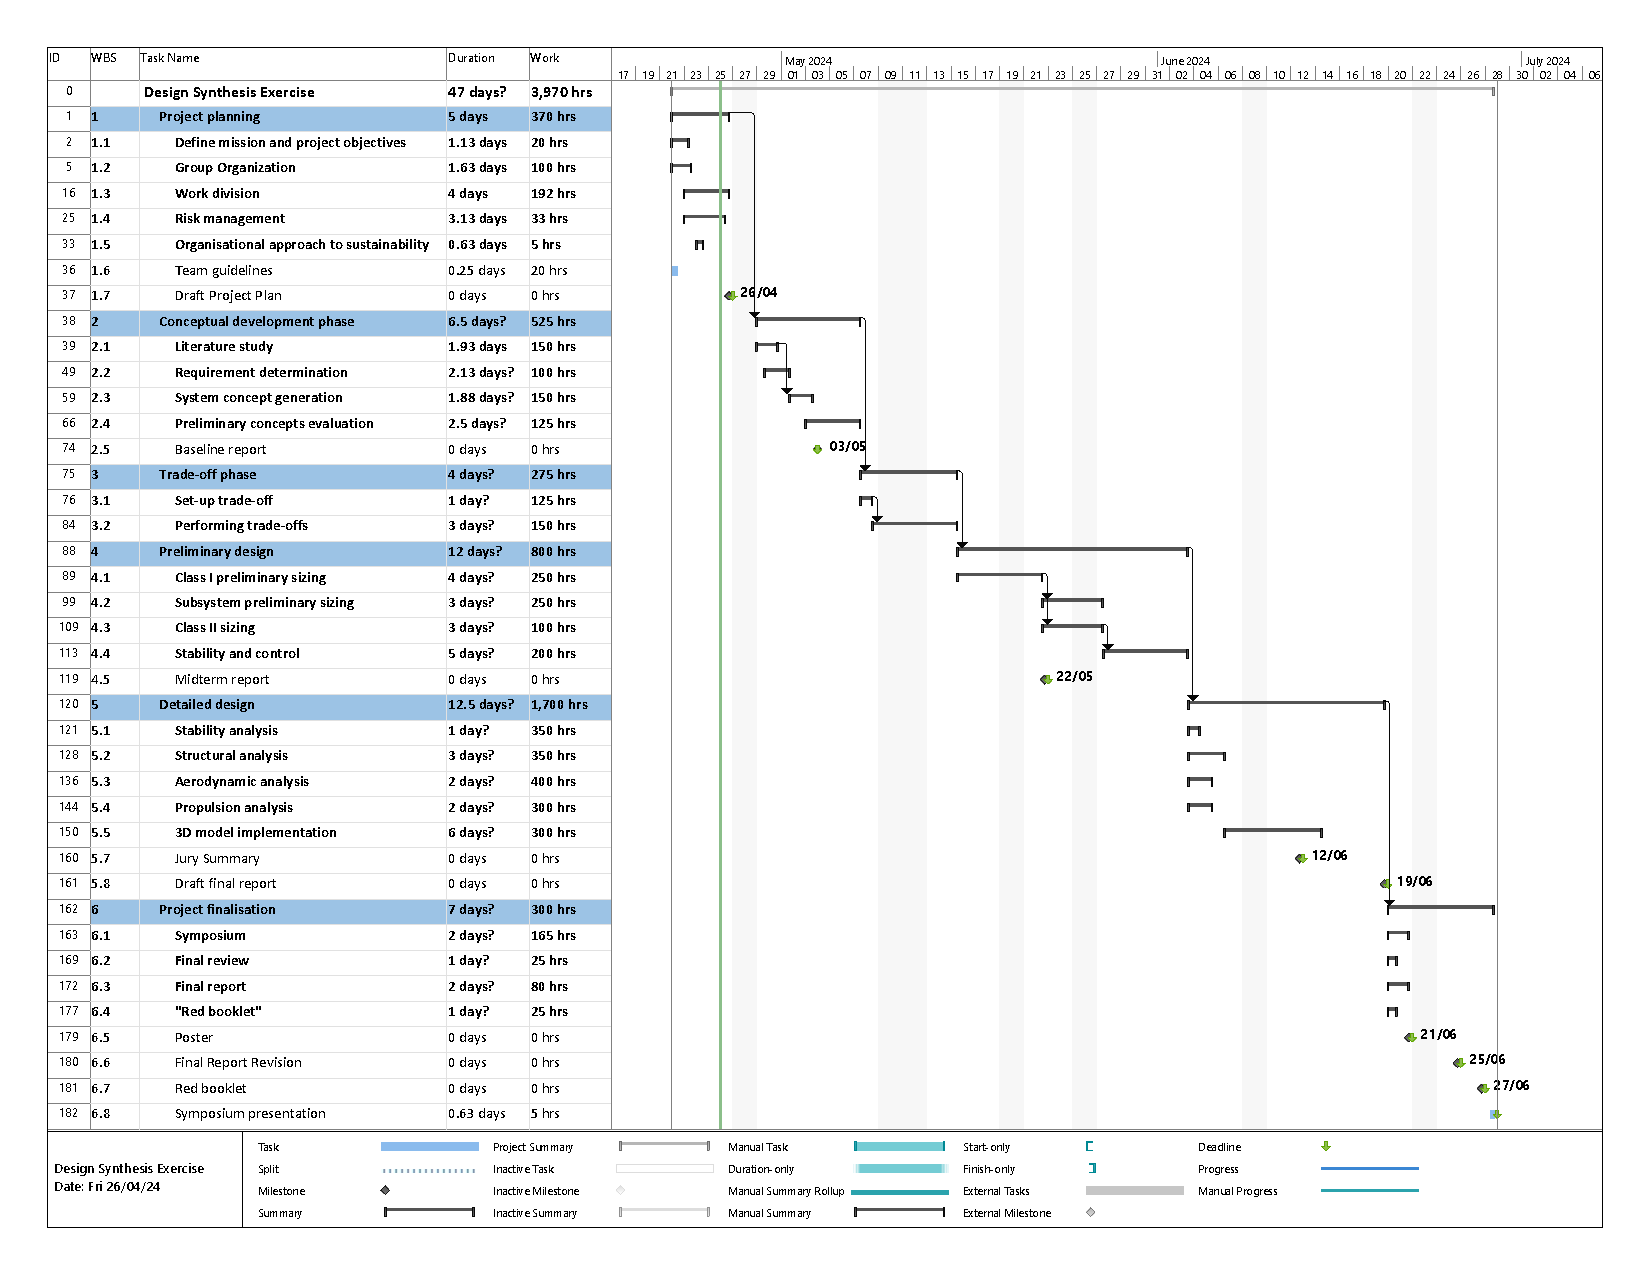
\includepdf{figures/AE3200-Gantt-chart-overall-26042024.pdf}
    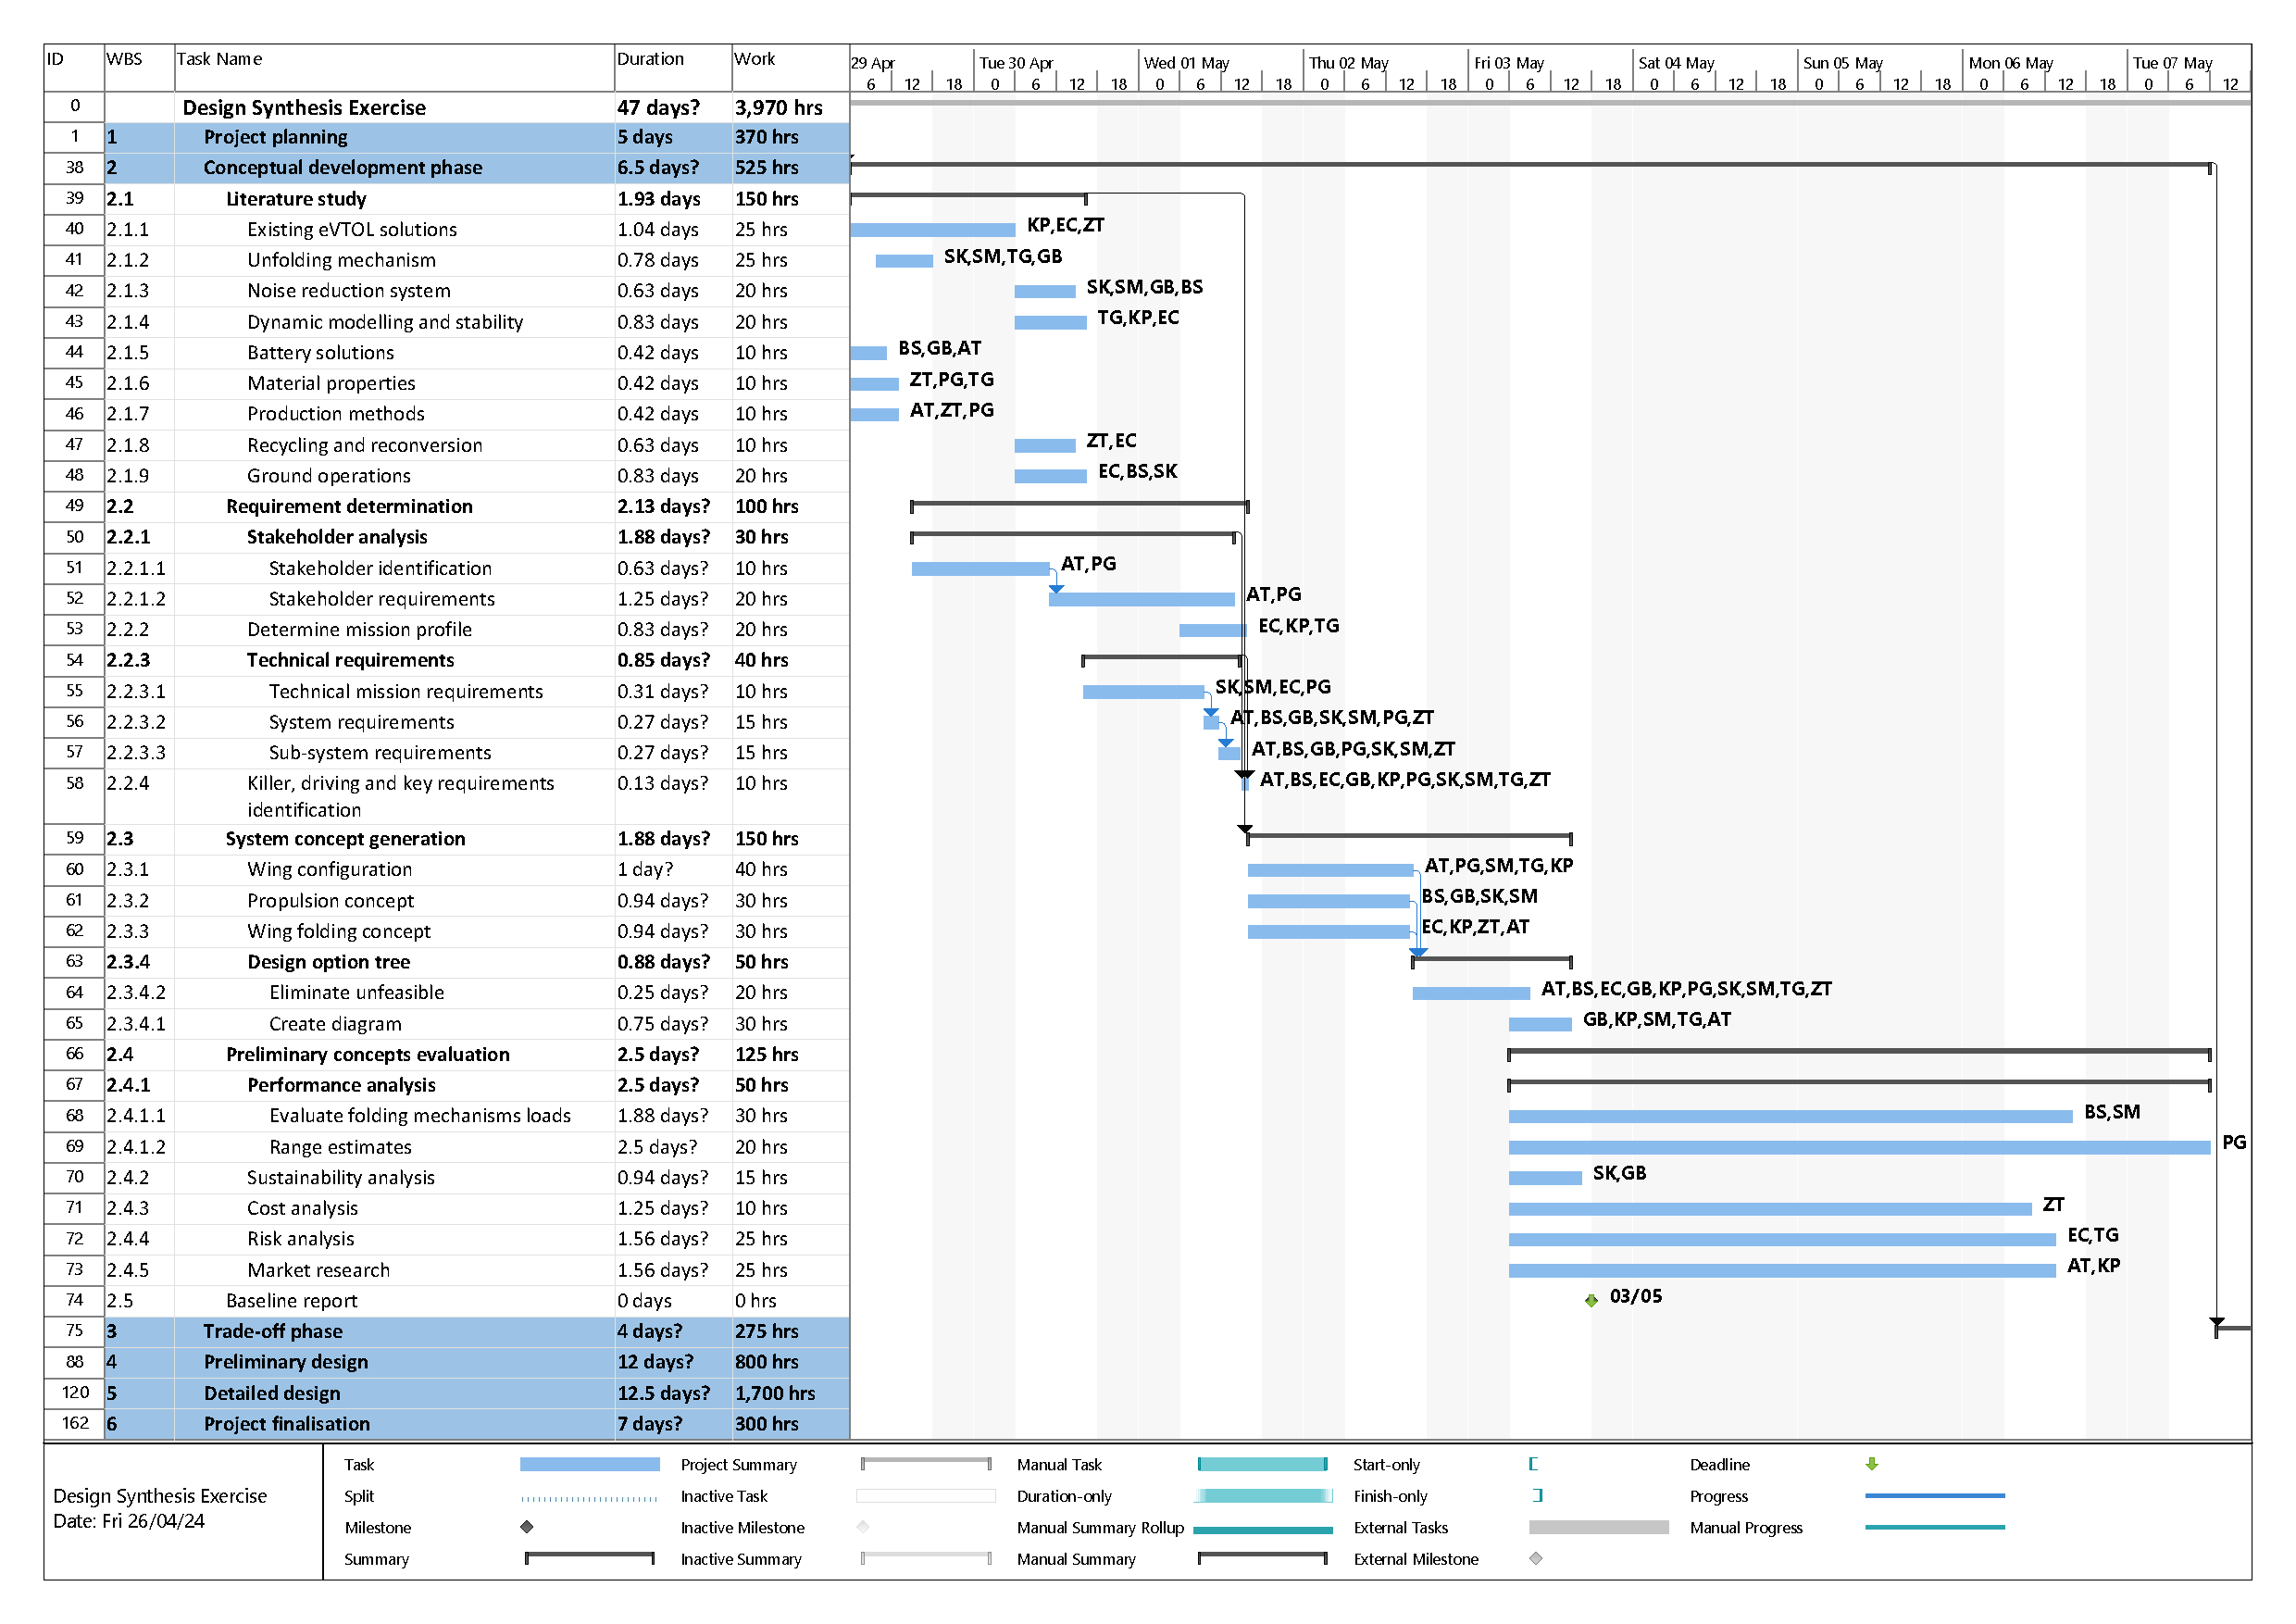
\includepdf{figures/AE3200-Gantt-chart-phase2-26042024.pdf}
    \KOMAoptions{paper=A4,paper=portrait,pagesize}
    \recalctypearea
}
\recalctypearea

\chapter{Project Guidelines}\label{ch:project_rules}
All team members agreed upon following a set of guidelines to ensure a smooth and efficient workflow during the DSE.
These guidelines are set up to ensure that all team members are on the same page and that the project is executed in a structured and organised manner, and are stated in the following sections.

\paragraph{Contact \& Communication}
\begin{itemize}
    \item The Communication Officer is responsible for formal contact with tutors, coaches and teaching assistants.
    \item Emails are written as a group and checked by the Communication Officer before being sent.
    \item Informal communication within the team will be done via WhatsApp.
\end{itemize}

\paragraph{Schedule}
\begin{itemize}
    \item The group shall be notified as soon as possible when a team member is aware of any absence during the DSE.
    \item When a team member arrives late to a session, he is obliged to bring a cake or something equivalent to the next session.
    \item A team member or work group shall notify the appropriate parties timely when running behind schedule.
    \item Everyone should feel encouraged to ask for help when deemed necessary.
\end{itemize}

\paragraph{Meeting}
\begin{itemize}
    \item During meetings, all team members are expected to give their attention fully, and thus no other work shall be executed simultaneously.
    \item Only English shall be spoken during the meetings and the entire project.
    \item At the start of the working day, a ten-minute stand-up meeting shall take place to:
    \begin{itemize}
        \item discuss the tasks and responsibilities of all individual team members;
        \item set up the whiteboard;
        \item assure that all team members are notified and conscious of the agenda of the meeting with the coaches.
    \end{itemize}
    \item At the end of the working day, a fifteen-minute shutdown meeting shall take place, where the tasks done for the day will be discussed and the timetable will be filled in.
\end{itemize}

\paragraph{Planning}
\begin{itemize}
    \item The Gantt Chart (\cref{sec:gantt-chart}) shall be used for the official planning of the project.
    \item Trello boards shall be used for day-to-day task generation and tracking.
    \item It is each team member’s responsibility to keep their tasks up to date on the Trello board and be informed of the tasks executed by other team members.
\end{itemize}

\paragraph{Documenting}
\begin{itemize}
    \item LaTeX shall be used for the generation of all report deliverables.
    \item All LaTeX projects shall be stored and versioned in GitHub, as well as on the Overleaf platform for the most recent version.
    \item Major versions of the report shall be exported as PDFs and stored in the directory named "Important reports versions" in the shared Microsoft Teams drive.
    \item The following LaTeX guidelines are set up, these shall be enforced by the documents manager and software manager:
    \begin{itemize}
        \item For notes, comments, and tasks within the LaTeX projects, the \verb|/TODO| package shall be utilised.
        Before handing in the report these \verb|/TODO| notes should be removed.
        \item Every chapter, section, figure, table, and equation shall be labelled.
        \item Every figure and table shall have a caption.
        \item Every figure shall be stored in the \verb|figures| directory, in a separate subdirectory for each chapter, and preferably as a PDF file or vector graphic.
        \item Every sentence shall start on a new line and paragraphs shall be divided by an empty line.
        \item For referencing, the \verb|cleveref| package shall be used.
        This entails the use of i.e\@. the \verb|\cref{}| and \verb|\Cref{}| commands.
        \item For numerical values and units the \verb|siunitx| package shall be used.
        This entails the use of i.e\@. the \verb|\qty{}{}| command.
        %    \item For acronyms and abbreviations the \verb|acronym| package shall be used.
        %    This entails the use of i.e\@. the \verb|\ac{}|, \verb|\Ac{}|, and \verb|\acf{}| commands.
    \end{itemize}
\end{itemize}

\paragraph{Language}
\begin{itemize}
    \item All deliverables shall be written in British English.
    \item The use of the passive voice and the first person shall be avoided in the report.
    \item During working hours only English is spoken.
    \item Make correct and frequent use of punctuation in the report.
\end{itemize}

\paragraph{Proofreading}
\begin{itemize}
    \item Clear proofreading guidelines start by adhering strictly to the documenting and language guidelines.
    \item The QAO shall assign all the team members with proofreading responsibilities, which consist of:
    \begin{itemize}
        \item Equal work per member.
        \item Each member being assigned to their expertise and familiarity.
    \end{itemize}
    \item Clear and realistic deadlines are set by the QAO, which consists of multiple rounds of proofreading.
    \item After the first proofreading round, each member proofreads a different chapter/section in a chronological order, and provides it with constructive feedback through comment features and discussion.
    \item Ensure consistency and accuracy by double-checking references and style/punctuation used.
    \item One more proofread round acts as a final review by all members of larger parts, to ensure an error-free and coherent report.
\end{itemize}

\paragraph{Code}
\begin{itemize}
    \item The Python programming language shall be used as much as possible for coding tasks.
    \item All code shall be stored and versioned in the GitHub repository.
    \item The code shall be written in a modular way, with functions, classes, and modules used to separate different parts of the code.
    \item All code shall be properly typed, with type hints used for all functions and classes.
    \item Further, the PEP8 coding standard shall be followed as much as possible.
    \item Each team member shall work in the appropriate branch of the repository.
    \item The Software Manager shall be responsible for merging the branches into the main branch, and overall code quality.
    \item For notes, comments, and tasks within the repository, the \verb|#todo| comment shall be utilised.
    \item For printing messages to the console, the \verb|logging| module shall be used.
    \item Standard functions, for i.e\@. the generation of plots and figures, shall be provided and utilised whenever possible.
\end{itemize}

\paragraph{Computer Aided Modelling (CAD)}
\begin{itemize}
    \item The naming convention (TBD) shall be respected and utilised for all parts and assemblies.
    \item Everything shall and must be iso-constrained.
    \item Whenever possible, parameterised design shall be utilised, since iteration and modification will be a critical part of the design process.
    \item It is encouraged to work in a highly modular manner, with parts and assemblies separated as much as possible.
    \item So-called planes shall be hidden when not in use, to avoid confusion and clutter in the design.
\end{itemize}

\paragraph{Artificial Intelligence}
\begin{itemize}
    \item No generative artificial intelligence shall be used to generate content intended for a deliverable in any way.
    \item Generative artificial intelligence shall not be used to perform or check calculations.
    \item Generative artificial intelligence may be used to generate code lines if, and only if, the generated code is fully understood.
\end{itemize}
\chapter{Organisational Risk Assessment}\label{ch:organisational-risk-assessment}
In this chapter, an organisational risk management plan will be made in order to assess and manage the relevant risks to the project.
In order to realise this risk management plan, a SWOT diagram is displayed and abbreviated on in \cref{sec:SWOT-Analysis}.
This diagram will be used as the input for the risk analysis in \cref{sec:Risk-Analysis}.


\section{SWOT Analysis}\label{sec:SWOT-Analysis}
A SWOT analysis is a planning tool that helps identify the Strengths and Weaknesses, which are internal aspects, and Opportunities and Threats, which are external aspects involved in the organisation.
In \cref{fig:swotanalysis} the SWOT diagram can be seen.
\begin{figure}[ht]
    \centering
    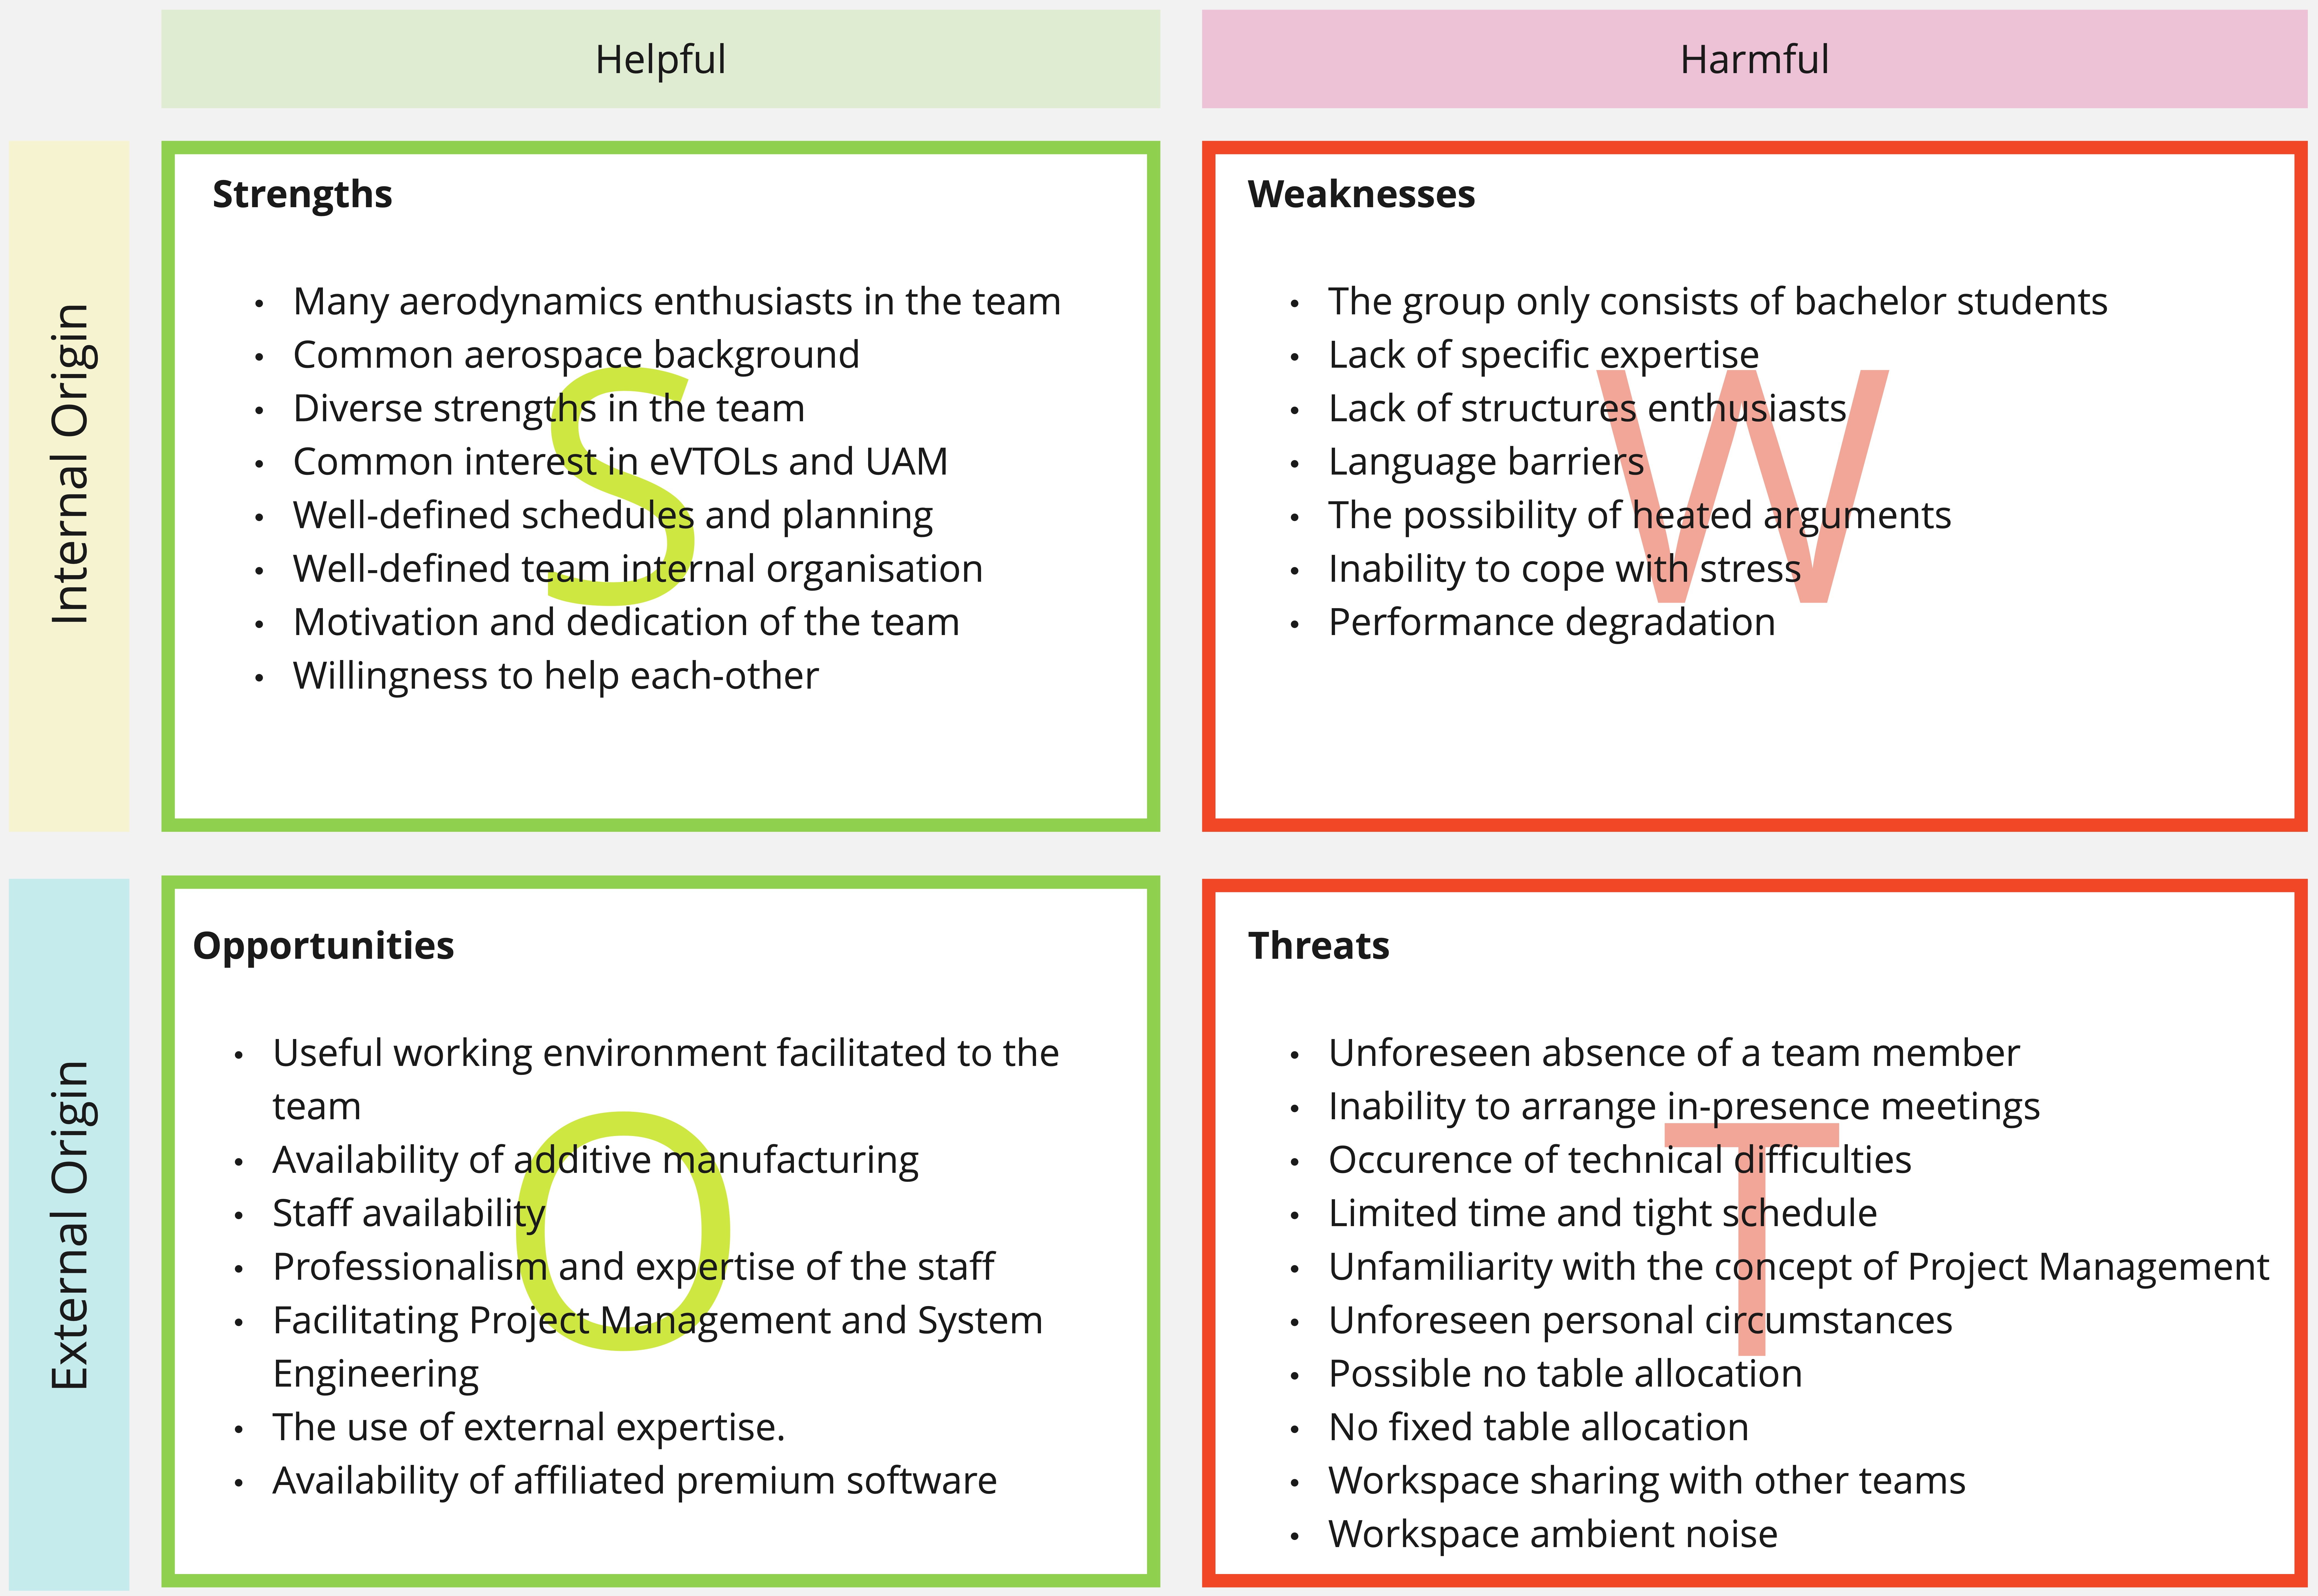
\includegraphics[width=\linewidth]{figures/Copy SWOT Analysis.jpg}
    \caption{SWOT Diagram}
    \label{fig:swotanalysis}
\end{figure}

This analysis is used to understand and identify potential organisational risks.
If a weakness is a threat as well, this is considered a serious risk, because an external threat induces problems.
If this is a team weakness, however, problems might arise if proper risk mitigation is not executed.


\section{Risk Analysis}\label{sec:Risk-Analysis}
This section presents the results of the risk analysis.
Firstly, in \cref{subsec:Risk-Metrics} the most important risks are identified, utilising the SWOT analysis.
During this analysis, the likelihood and the scheduled impact of the risk are determined, which will result in a final score.
Next, the risk register and map are constructed in \cref{subsec:Risk-Register-and-Map} to assist risk mitigation and contingency planning.
Thereafter, the mitigation strategy and contingency plan are proposed in \cref{subsec:Risk-Mitigation-and-Contingency-Plan} to decrease the likelihood and impact of the risk.
Finally, the mitigated risk register and map are presented in \cref{tab:mitriskregister,fig:riskmaps}.

\subsection{Risk Metrics}\label{subsec:Risk-Metrics}
Before the risk events can be identified and quantified a metrics system shall be defined.
A risk event has two distinguishable properties, the likelihood and the impact of an event on the project.
These two properties are quantified on a scale range of 1 to 5.
The description of the two metrics are summarised in \cref{tab:likelihood_metrics,tab:impact_metrics}.

\begin{table}[ht]
    \centering

    \begin{minipage}{0.5\textwidth}
        \centering
        \begin{tabular}{ccc}
            \hline
            Likelihood & Description & Probability         \\ \hline
            5          & Very High   & $0.7\leq P$         \\
            4          & High        & $ 0.5 \leq P < 0.7$ \\
            3          & Moderate    & $0.3 \leq P < 0.5$  \\
            2          & Low         & $0.05 \leq P < 0.3$ \\
            1          & Very Low    & $P < 0.05$          \\ \hline
        \end{tabular}
        \caption{Likelihood metrics}
        \label{tab:likelihood_metrics}
    \end{minipage}\hfill
    \begin{minipage}{0.5\textwidth}
        \centering
        \begin{tabular}{cc}
            \hline
            Impact & Description  \\ \hline
            5      & Catastrophic \\
            4      & Critical     \\
            3      & Marginal     \\
            2      & Acceptable   \\
            1      & Negligible   \\ \hline
        \end{tabular}
        \caption{Impact metrics}
        \label{tab:impact_metrics}
    \end{minipage}
\end{table}

\subsection{Risk Register and Map}\label{subsec:Risk-Register-and-Map}
An efficient way of risk identification and handling is the generation of a risk register and map.
The investigation of the risk events employed the results of the SWOT analysis in \cref{sec:SWOT-Analysis}. Different phases of the project were considered to identify the major risk events.
For each phase, several planning risk categories were recognised.
These entail: organizational, schedule, communication, internal, external and resource.
All categories were broken down into several risk events. Subsequently, the impacts were described and quantified alongside the likelihood.
Finally, the risk was quantified as the product of the normalised likelihood and the impact.
The resulting risk register of the risk investigation is depicted in \cref{tab:mitriskregister}.

All the unmitigated risks stated in \cref{tab:unmitigated_risk_map}, can be plotted into a risk map, which can be seen in \cref{fig:unmitigated}.
The map visualizes the severity of the risk and gives an easy overview of which risks need to be mitigated.
For example, it can be seen that R-G-6 and R-G-7 require a mitigation strategy, because they are positioned in the red top-right zone of \cref{fig:unmitigated}.
\begin{table}[ht]
\caption{Unmitigated organizational risk register}
    \label{tab:unmitigated_risk_map}
    \centering
    \resizebox{\linewidth}{!}{
        \begin{tabular}{lclllccc}
            \hline
            \multicolumn{1}{c}{\multirow{2}{*}{Risk ID}} & \multirow{2}{*}{Period} & \multicolumn{1}{c}{\multirow{2}{*}{Category}}                    & \multicolumn{1}{c}{\multirow{2}{*}{Risk Description}}                                                           & \multicolumn{1}{c}{\multirow{2}{*}{Impact Description}}                                     & \multicolumn{3}{c}{Unmitigated Risk}                                               \\
            \cline{6-8}
            \multicolumn{1}{c}{} & & \multicolumn{1}{c}{} & \multicolumn{1}{c}{}                 & \multicolumn{1}{c}{}                                                                        & \multicolumn{1}{l}{Likelihood} & Impact & Risk                                     \\ \hline
            R-G-1 & \multirow{8}{*}{All} & Schedule & \begin{tabular}[c]{@{}l@{}}
                                                          Incorrect time allocation, \\insufficient time is given for tasks
            \end{tabular} & Accumulated Delays & 4 & 4 & {\cellcolor[rgb]{0.502,0.541,0.533}}3.2 \\
            R-G-2 & & Schedule & Unforeseen absence of a team member & \begin{tabular}[c]{@{}l@{}}
                                                                           Decreased working\\capacity
            \end{tabular}                & 2 & 5             & {\cellcolor[rgb]{0.545,0.776,0.471}}2    \\
            R-G-3                & & Schedule             & interdependencies of tasks~ & \begin{tabular}[c]{@{}l@{}}
                                                                                              Decreased working \\efficiency\\and increased time~
            \end{tabular} & 5 & 3 & {\cellcolor[rgb]{0.51,0.58,0.522}}3 \\
            R-G-4                & & External        & Unavailability of tutors, coaches          & Increased uncertainity & 2                              & 3      & {\cellcolor[rgb]{0.239,0.898,0.714}}1.2   \\
            R-G-5 & & External & Unavailability of~ teacher assistant & Increased uncertainity & 1 & 2 & {\cellcolor[rgb]{0.082,0.922,0.843}}0.4 \\
            R-G-6 & & Schedule & \begin{tabular}[c]{@{}l@{}}
                                     Inability to arrange in-presence \\meetings when no table is available
            \end{tabular} & \begin{tabular}[c]{@{}l@{}}
                                Decreased communication\\and working~efficiency
            \end{tabular} & 4 & 5 & {\cellcolor[rgb]{0.475,0.384,0.573}}4 \\
            R-G-7 & & Communication & \begin{tabular}[c]{@{}l@{}}
                                          Inadequate communication\\~between team members and roles
            \end{tabular} & \begin{tabular}[c]{@{}l@{}}
                                Working parallel on\\the same task
            \end{tabular} & 4 & 5 & {\cellcolor[rgb]{0.475,0.384,0.573}}4 \\
            R-G-8 & & Communication & Working space distractions~ & Decreased work quality & 5 & 1 & {\cellcolor[rgb]{0.082,0.922,0.843}}1 \\ \hline
            R-P-1 & \multirow{4}{*}{\begin{tabular}[c]{@{}c@{}}
                                        Project\\Planning
            \end{tabular}} & Internal & Unfamiliarity with Project Management & \begin{tabular}[c]{@{}l@{}}
                                                                                    Slow project planning\\progress
            \end{tabular} & 3 & 4 & {\cellcolor[rgb]{0.529,0.698,0.49}}2.4 \\
            R-P-2 & & Internal & Lack of all needed range of expertise & \begin{tabular}[c]{@{}l@{}}
                                                                             Decreased personal\\motivation
            \end{tabular} & 5 & 3 & {\cellcolor[rgb]{0.51,0.58,0.522}}3 \\
            R-P-3 & & Organizational & \begin{tabular}[c]{@{}l@{}}
                                           Unimplemented risk mitigation\\by the responsible members
            \end{tabular} & Unsupervised risks & 3 & 5 & {\cellcolor[rgb]{0.51,0.58,0.522}}3 \\
            R-P-4 & & Organizational & \begin{tabular}[c]{@{}l@{}}
                                           Excessive expectations are set \\during project planning
            \end{tabular} & Accumulated Delays & 4 & 3 & {\cellcolor[rgb]{0.529,0.698,0.49}}2.4 \\ \hline
            R-C-1 & \begin{tabular}[c]{@{}c@{}}
                        Conceptual\\~phase
            \end{tabular} & Schedule & \begin{tabular}[c]{@{}l@{}}
                                           Unable to come up with sufficient \\number of feasible concepts
            \end{tabular} & \begin{tabular}[c]{@{}l@{}}
                                Less optimal solution\\outcome
            \end{tabular} & 3 & 2 & {\cellcolor[rgb]{0.239,0.902,0.714}}1.2 \\ \hline
            R-T-1 & \begin{tabular}[c]{@{}c@{}}
                        Trade-off \\Phase
            \end{tabular} & Schedule & \begin{tabular}[c]{@{}l@{}}
                                           Unable to complete the trade-off\\and conclude the final design concept
            \end{tabular} & \begin{tabular}[c]{@{}l@{}}
                                Delay in preliminary and\\detailed design
            \end{tabular} & 2 & 5 & {\cellcolor[rgb]{0.545,0.776,0.471}}2 \\ \hline
            R-PD-1 & \begin{tabular}[c]{@{}c@{}}
                         Preliminary\\Design
            \end{tabular} & Schedule & \begin{tabular}[c]{@{}l@{}}
                                           Insufficient number iterations for\\the preliminary design
            \end{tabular} & \begin{tabular}[c]{@{}l@{}}
                                Limited time for detail\\design
            \end{tabular} & 3 & 4 & {\cellcolor[rgb]{0.529,0.698,0.49}}2.4 \\ \hline
            P-D-1 & \multirow{2}{*}{\begin{tabular}[c]{@{}c@{}}
                                        Detailed\\Design
            \end{tabular}} & Schedule & Unable to validate the final design on time & Incompleted project & 2 & 5 & {\cellcolor[rgb]{0.545,0.776,0.471}}2 \\
            P-D-2 & & Resorce & Insufficient resources for 3D prototype & \begin{tabular}[c]{@{}l@{}}
                                                                              Missing prototype\\for final review
            \end{tabular} & 2 & 5 & {\cellcolor[rgb]{0.545,0.776,0.471}}2 \\\hline
            R-R-1 & \multirow{3}{*}{Documenting} & \begin{tabular}[c]{@{}l@{}}
                                                       \\External
            \end{tabular} & \begin{tabular}[c]{@{}l@{}}
                                Document crashing, \\accidental deleting, etc.~
            \end{tabular} & \begin{tabular}[c]{@{}l@{}}
                                Loss of progress, \\or even work
            \end{tabular} & 2 & 5 & {\cellcolor[rgb]{0.545,0.776,0.471}}2 \\
            R-R-2 & & Organizational & Unorganised or parallel proofreading~ & \begin{tabular}[c]{@{}l@{}}
                                                                                   Some parts not proofread,\\~or double work division
            \end{tabular} & 4 & 3 & {\cellcolor[rgb]{0.529,0.698,0.49}}2.4 \\
            R-R-3 & & Communication~ & \begin{tabular}[c]{@{}l@{}}
                                           Misfocusses on the language\\and style used in documents
            \end{tabular} & \begin{tabular}[c]{@{}l@{}}
                                Increase time spent\\on document~
            \end{tabular} & 4 & 1 & {\cellcolor[rgb]{0.082,0.922,0.843}}0.8 \\
            \arrayrulecolor{black}\hline
        \end{tabular}}
    
\end{table}

\subsection{Risk Mitigation and Contingency Plan}\label{subsec:Risk-Mitigation-and-Contingency-Plan}
% Explain what the likelihood and consequence mean in the risk map
%mitigation strategy and a contingency plan if the risk occurs
%Two risk maps
%Pre mitigation
%Post mitigation
A plan is proposed to decrease the probability of the occurrence of risk events and, in case a risk event cannot be avoided, reduce the impact of the event.
The plan consists of two phases a risk mitigation and a contingency plan decreasing the likelihood and the impact respectively.
It is important to note that for each mitigation strategy and contingency plan one member is chosen to be responsible, in order to even out the burden and ensure focus on each risk.
Furthermore, after all the measures taken, the mitigated likelihood and impact after described in a table afterwards, of which a mitigated risk map can be created.

\textbf{R-G-1 (Project Manager)}:
\newline Mitigation strategy: Active management by the PM.
\newline Contingency plan: Immediately notify the PM if a deadline seems infeasible.


\textbf{R-G-2 (Project Manager)}:
\newline Mitigation strategy: Adhere to the so-called "cake rule", as well as the expulsion of the project after two missed sessions.
\newline Contingency plan: Redistribute the workload of the missing team member on the missed day, possibly assigning compensational tasks for the missing member.

\textbf{R-G-3 (Quality Assurance Officer)}:
\newline Mitigation strategy: Establish clear communication and collaboration lines between members.
\newline Contingency plan: Identify the problem with members involved and update the communication- and collaboration lines between members.

\textbf{R-G-4 (Communication Officer)}:
\newline Mitigation strategy: Set clear communication guidelines and routines with tutors and coaches.
\newline Contingency plan: Contact tutors or coaches with important questions through other means of communication such as teams or email.

\textbf{R-G-5 (Communication Officer)}:
\newline Mitigation strategy: Set clear communication guidelines and routines with teaching assistants.
\newline Contingency plan: Contact teaching assistants with important questions through other means of communication such as teams or email.

\textbf{R-G-6 (Secretary)}:
\newline Mitigation strategy: Plan to reserve tables at another place in advance.
\newline Contingency plan: Meet through any online alternative and come up with a clear agenda for the next physical meeting.

\textbf{R-G-7 (Chairman)}:
\newline Mitigation strategy: Frequent meetings and discussions among the team, in order to be continuously on the same page.
\newline Contingency plan: Gather as a whole and clearly communicate improvements that need to be taken.

\textbf{R-G-8 (Communication Officer)}:
\newline Mitigation strategy: Set working space boundaries and rules with other teams in the room.
\newline Contingency plan: Clearly communicate space boundaries and rules with other teams in the room.

\textbf{R-P-1 (Project Manager)}:
\newline Mitigation strategy: As all the team members are new to project management, it can be seen as taking the risk.
\newline Contingency plan: Actively research and implement project management strategies

\textbf{R-P-2 (Systems Engineer)}:
\newline Mitigation strategy: Attempt to allocate everyone to their preferred roles and tasks.
\newline Contingency plan: Allocating people to both preferred and needed roles and tasks as a compromise.

\textbf{R-P-3 (Risk Manager)}:
\newline Mitigation strategy: Frequent risk map update and risk management reminders
\newline Contingency plan: Adjust the contigency plan accordingly and update the risk map

\textbf{R-P-4 (Project Manager)}:
\newline Mitigation strategy: Trying to set feasable expectations in the project planning.
\newline Contingency plan: Adjust the project plan where needed and learn from made mistakes.

\textbf{R-C-1 (Systems Engineer)}:
\newline Mitigation strategy: Prepare a well-defined concept planning and openly brainstorm with the whole group.
\newline Contingency plan: Change the concept planning and re-define the possibilities each concept brings.

\textbf{R-T-1 (Systems Engineer)}:
\newline Mitigation strategy: Make sure all memebers of the group come well-prepraed in order to decide.
\newline Contingency plan: Stop work and make sure all members are on the same page, if needed work over-time.

\textbf{R-PD-1 (Systems Engineer)}:
\newline Mitigation strategy: Prepare a proper iteration plan, as well as having clear connections between responsible members.
\newline Contingency plan: If the team members have enough time; make an improved iteration plan, else make use of approximations

\textbf{R-D-1 (Project Manager)}:
\newline Mitigation strategy: Propose resource and cost plan, so what resource is needed when.
\newline Contingency plan: By looking at the plan tackle the most important problems and consider working over-time.

\textbf{R-D-2 (Cost Manager)}:
\newline Mitigation strategy: Plan early-on which parts of the project will be 3D-printed, and carefully watch time spent is consistent with plan.
\newline Contingency plan: Decide on the most important parts to be 3D-printed.

\textbf{R-R-1 (Documents Manager)}:
\newline Mitigation strategy: Making informed use of software, use collaborative software environments.
\newline Contingency plan: Stop work with members involved and carefully come up with a proper solution.

\textbf{R-R-2 (Quality Assurance Officer)}:
\newline Mitigation strategy: Come up with a well-structured and -defined proofread plan the team can adhere to.
\newline Contingency plan: Gather the team together in order to be on the same page and adjust the proofread plan accordingly.

\textbf{R-R-3 (Quality Assurance Officer)}:
\newline Mitigation strategy: Establish clearly specified language guidelines.
\newline Contingency plan: Correct it and comment on it in the daily meeting, to prevent further mistakes.\\


These mitigation strategies decrease the likelihood, whereas the contingency plans decrease the impact, resulting in a decrease of the risk. This updates the risk register and map, as can be seen in \cref{tab:mitriskregister,fig:riskmaps}.
It clearly shows the shift of the risks leftwards and downwards, due to the mitigation strategy.
However, there are still outliers, namely R-P-3, R-P-2, R-G-7 and R-G-3, which still have a relatively high-risk value.
Therefore these risks are monitored by the designated person to ensure that the project progress does not halt.

\begin{table}[ht]
    \caption{Mitigated risk register}
    \label{tab:mitriskregister}
    \centering
    \resizebox{\linewidth}{!}{\begin{tabular}{lcclcccclc}
                                  \hline
                                  \multicolumn{1}{c}{ID} & \begin{tabular}[c]{@{}c@{}}
                                                               Mitigated\\Likelihood
                                  \end{tabular} & \begin{tabular}[c]{@{}c@{}}
                                                      Mitigated\\Impact
                                  \end{tabular} & Risk & Responsible Member & ID & \begin{tabular}[c]{@{}c@{}}
                                                                                       Mitigated \\Likelihood
                                  \end{tabular} & \begin{tabular}[c]{@{}c@{}}
                                                      Mitigated \\Impact
                                  \end{tabular} & Risk & \multicolumn{1}{c}{Responsible Member} \\ \hline
                                  R-G-1 & 2 & 3 & {\cellcolor[rgb]{0.553,0.82,0.459}}1.2 & Project Manager (Bradut)             & R-P-3 & 2                                                              & 4                                                          & {\cellcolor[rgb]{0.541,0.753,0.475}}1.6 & Risk Manager (Zoli)                     \\
                                  R-G-2 & 1 & 3 & {\cellcolor[rgb]{0.082,0.922,0.843}}0.6 & Project Manager (Bradut)                  & R-P-4 & 3 & 2 & {\cellcolor[rgb]{0.553,0.82,0.459}}1.2  & Project Manager (Bradut)                \\
                                  R-G-3 & 4 & 2 & {\cellcolor[rgb]{0.541,0.753,0.475}}1.6 & Quality Assurance Officer (Stefano)                      & R-C-1 & 2 & 2 & {\cellcolor[rgb]{0.082,0.922,0.843}}0.8 & Systems Engineer (Gregorio)             \\
                                  R-G-4 & 1 & 2 & {\cellcolor[rgb]{0.082,0.922,0.843}}0.4 & Communication Officer
                                  (Alessandro) & R-T-1 & 1                                                              & 3                                                          & {\cellcolor[rgb]{0.082,0.922,0.843}}0.6 & Systems Engineer (Gregorio)             \\
                                  R-G-5 & 1 & 1 & {\cellcolor[rgb]{0.082,0.922,0.843}}0.2  & Communication Officer
                                  (Alessandro)            & R-PD-1 & 2                                                              & 3                                                          & {\cellcolor[rgb]{0.553,0.82,0.459}}1.2  & Systems Engineer (Gregorio)             \\
                                  R-G-6 & 1 & 3 & {\cellcolor[rgb]{0.082,0.922,0.843}}0.6 & Secretary (Philip)         & P-D-1 & 1                                                              & 4                                                          & {\cellcolor[rgb]{0.082,0.922,0.843}}0.8 & Project Manager (Bradut)                \\
                                  R-G-7 & 3 & 3 & {\cellcolor[rgb]{0.537,0.722,0.482}}1.8 & Chairman (Tim)         & P-D-2 & 1 & 4 & {\cellcolor[rgb]{0.082,0.922,0.843}}0.8 & Cost Manager (Koen) \\
                                  R-G-8 & 3 & 1 & {\cellcolor[rgb]{0.082,0.922,0.843}}0.6 & Communication Officer (Alessandro)         & R-R-1 & 1 & 3 & {\cellcolor[rgb]{0.082,0.922,0.843}}0.6 & Documents Manager (Koen) \\
                                  R-P-1 & 3 & 2 & {\cellcolor[rgb]{0.553,0.82,0.459}}1.2 & Project Manager (Bradut)         & R-R-2 & 2 & 1 & {\cellcolor[rgb]{0.082,0.922,0.843}}0.4 & Quality Assurance Officer (Stefano) \\
                                  R-P-2 & 3 & 3 & {\cellcolor[rgb]{0.537,0.722,0.482}}1.8 & Systems Engineer (Gregorio)         & R-R-3 & 3 & 1 & {\cellcolor[rgb]{0.082,0.922,0.843}}0.6 & Quality Assurance Officer (Stefano) \\ \hline
    \end{tabular}}
    
\end{table}


\begin{figure}[ht]
    \centering
    \begin{subfigure}[b]{0.45\linewidth}
        \centering
        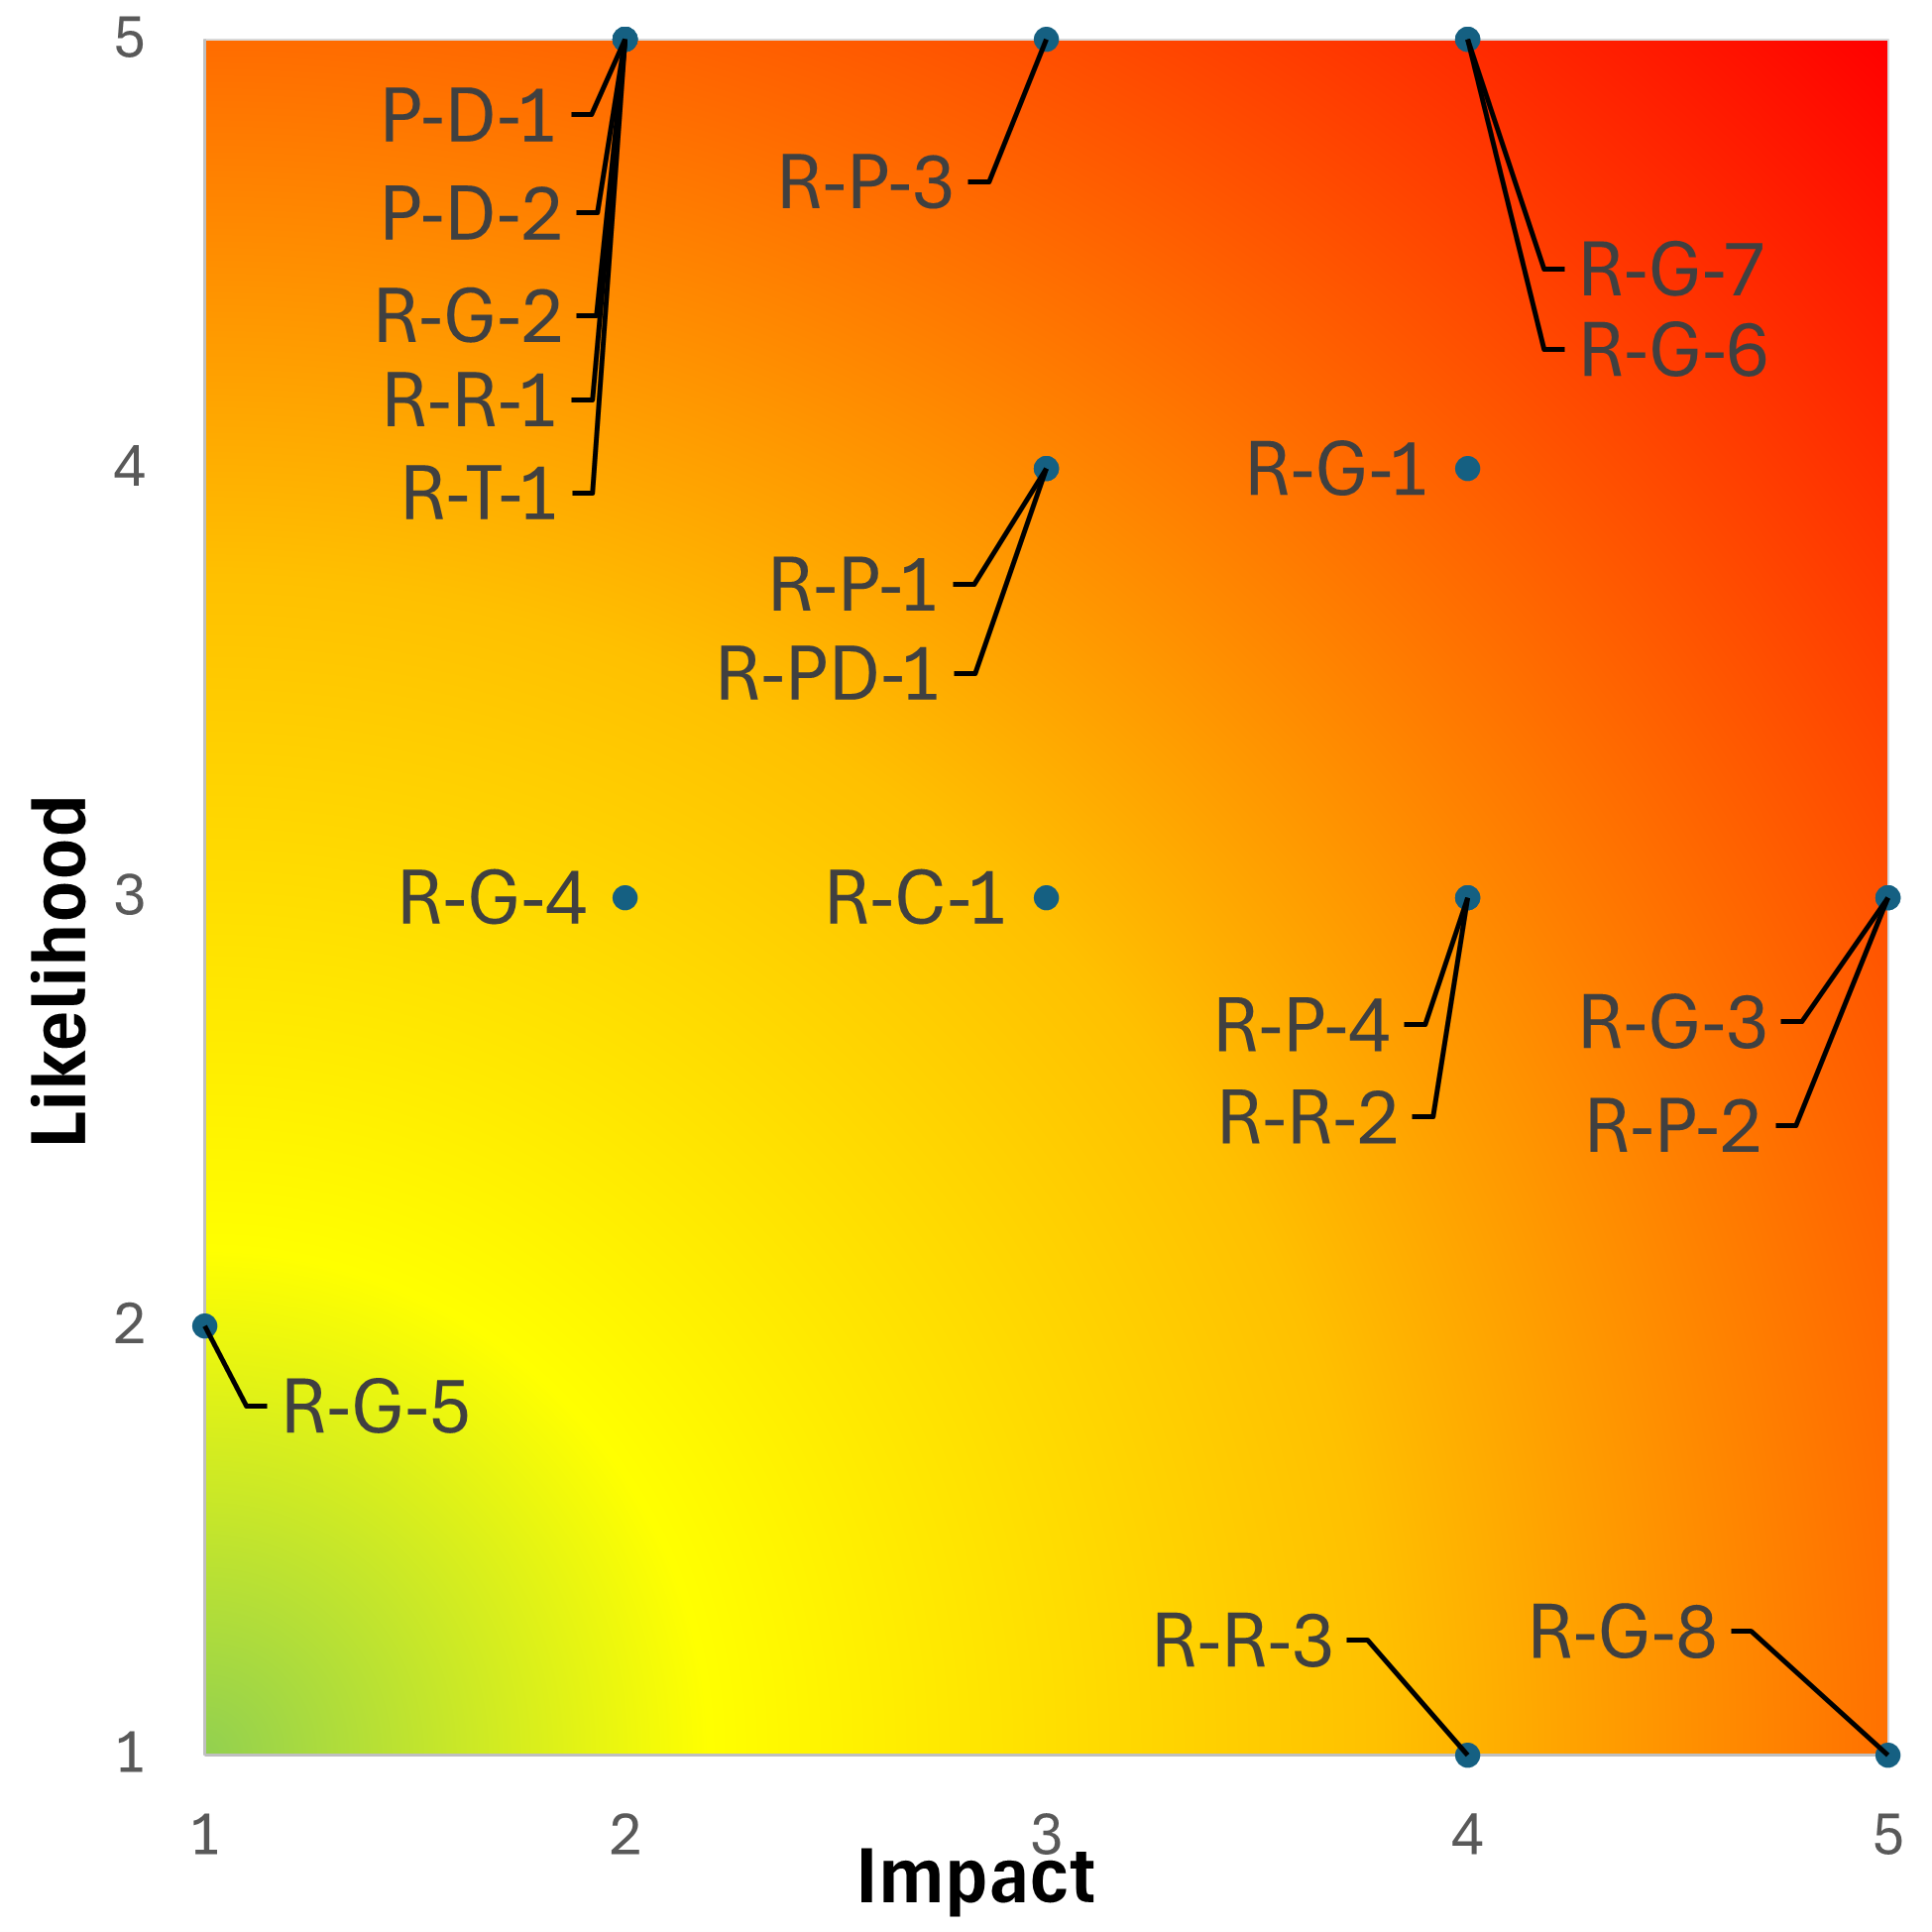
\includegraphics[width=\linewidth]{figures/Risk_map_unmitigated.png}
        \caption{Unmitigated risk map}
        \label{fig:unmitigated}
    \end{subfigure}
    \hspace{0.05\linewidth} % Adjust the spacing between the subfigures
    \begin{subfigure}[b]{0.45\linewidth}
        \centering
        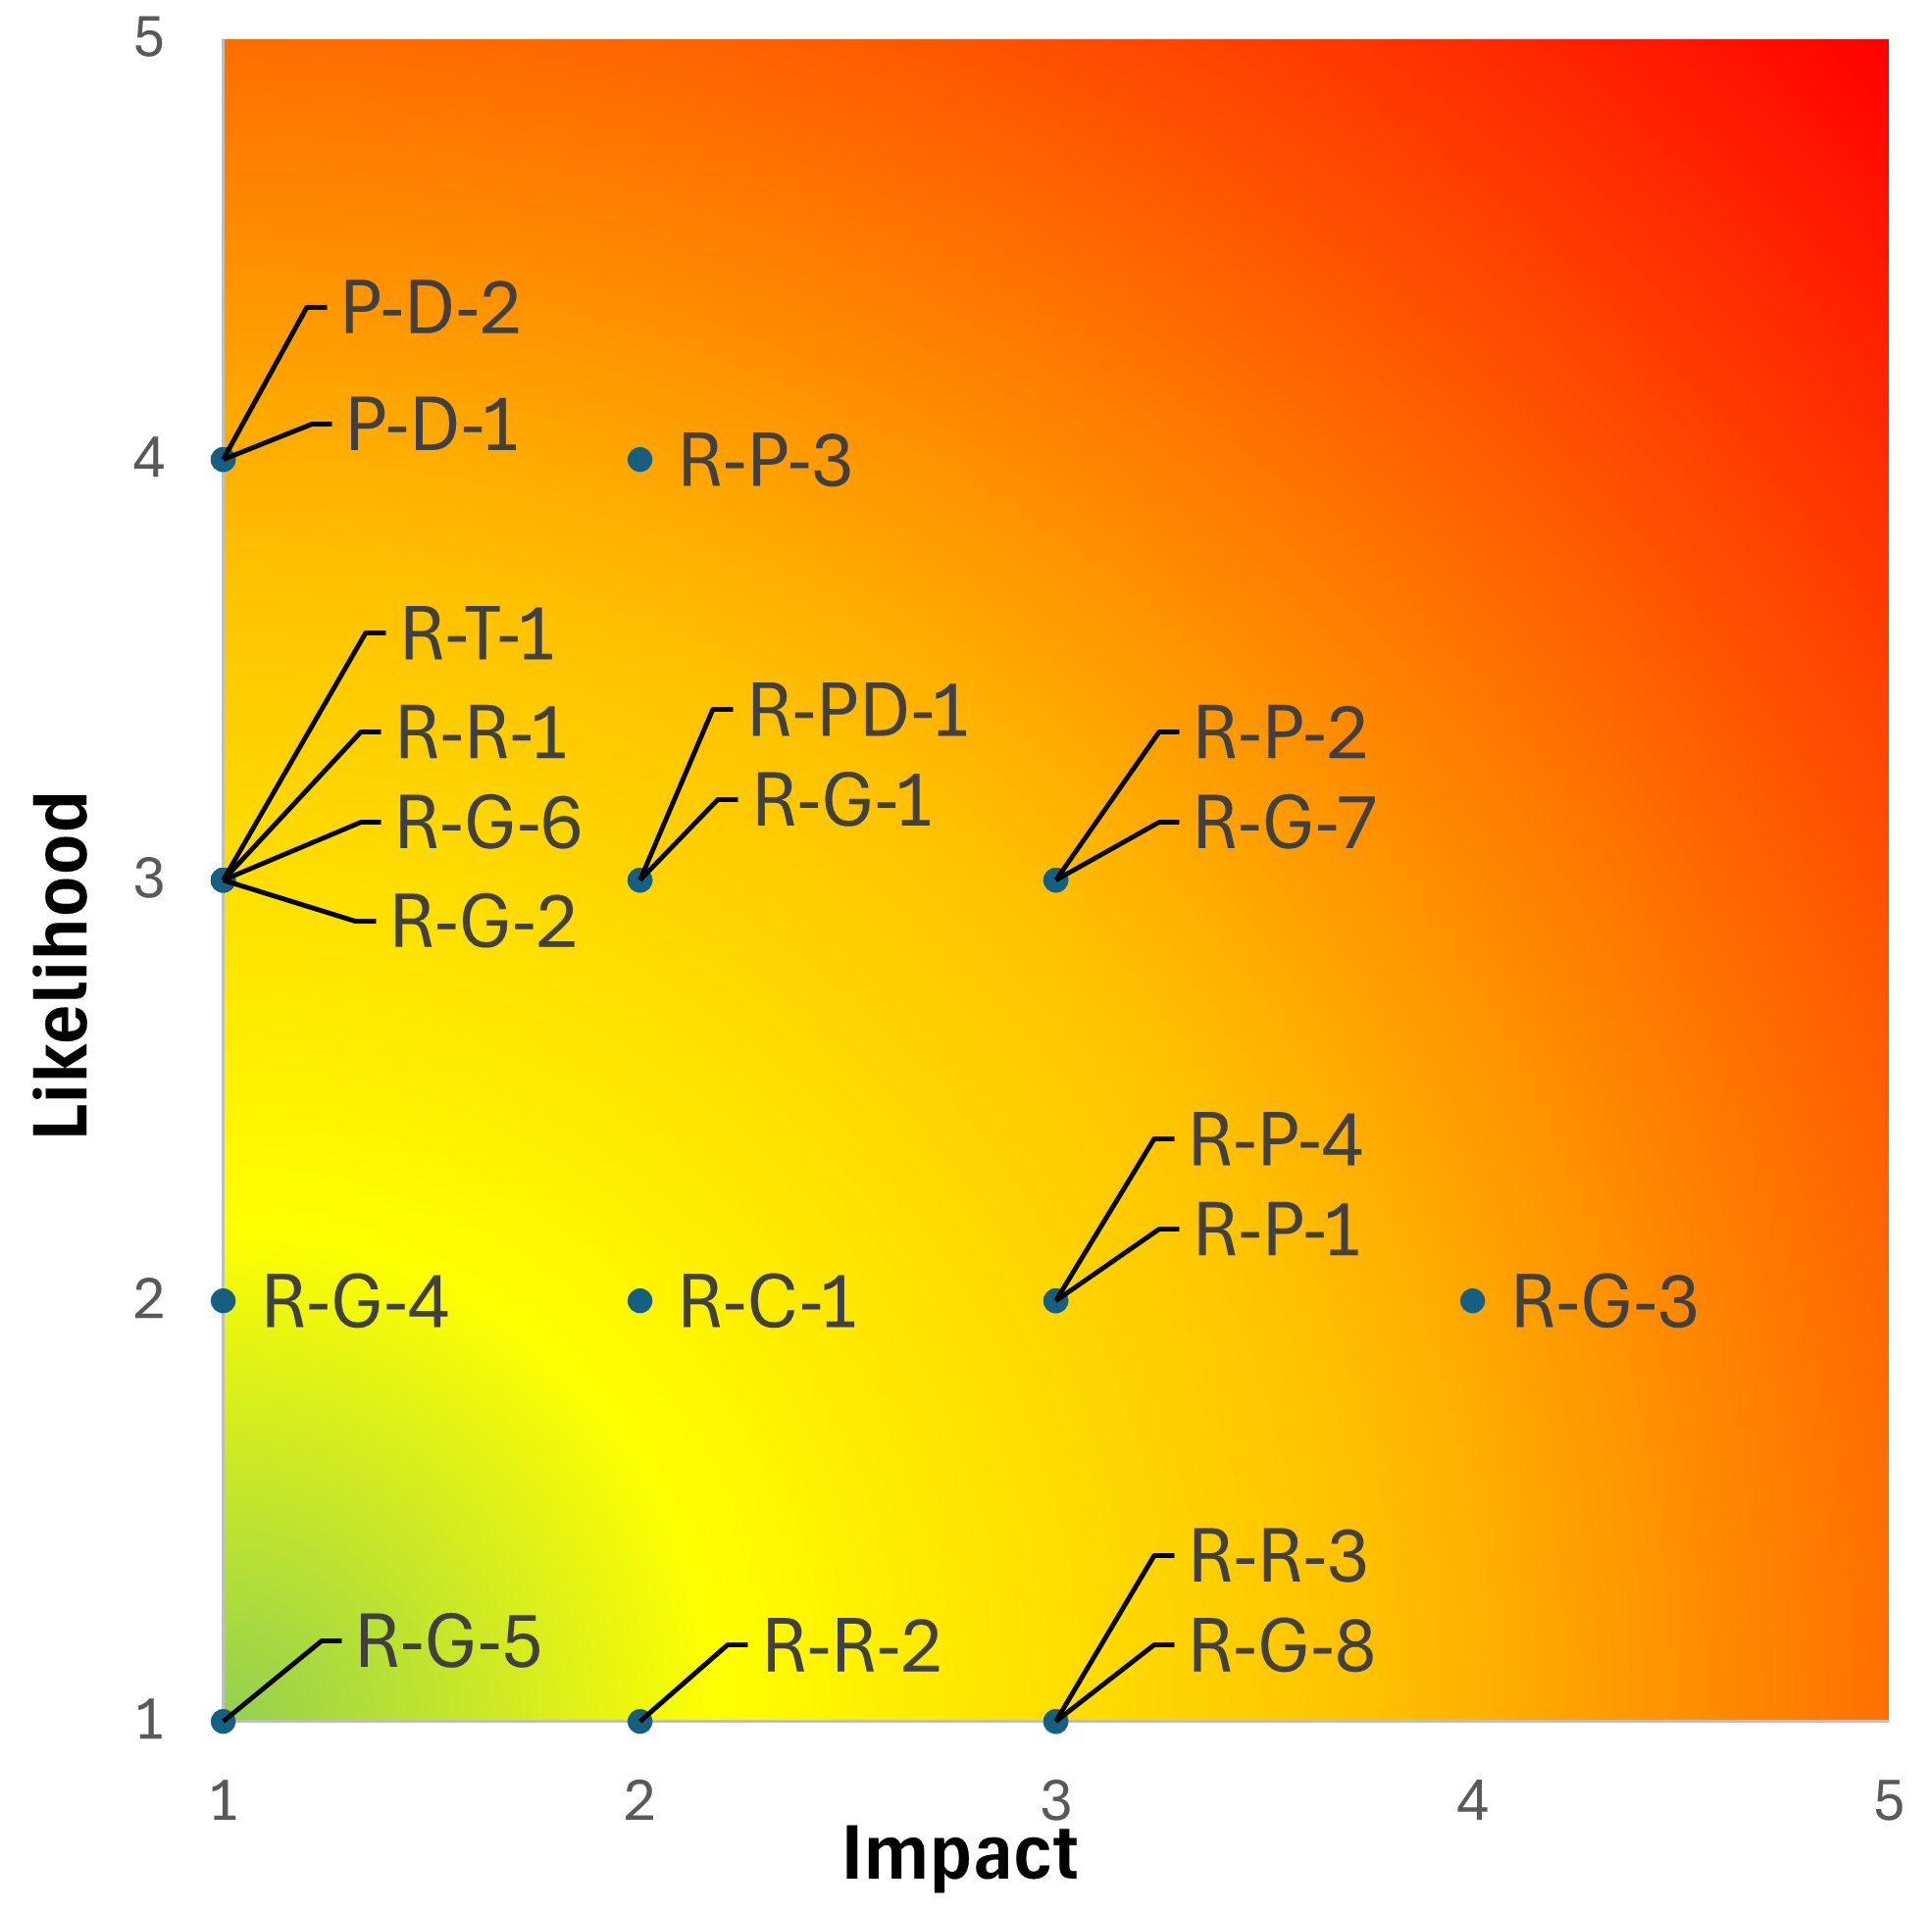
\includegraphics[width=\linewidth]{figures/Risk_map_mitigated.png}
        \caption{Mitigated risk map}
        \label{fig:mitigated}
    \end{subfigure}
    \caption{Comparison of unmitigated and mitigated risk maps}
    \label{fig:riskmaps}
\end{figure}
\chapter[Sustainability]{Approach to Sustainable Development}\label{ch:sustainability}
Now that the project phases have been carefully planned, and the group organisational structure determined, this chapter focuses on the measures taken within the group to allow sustainable development. 
World institutions such as the United Nations have increasingly highlighted sustainable behaviours in the past decades.
The seventeen sustainable development goals established by the UN in 2016 are a call to the world to promote prosperity, while protecting the planet.
The broadness and multifaceted nature of sustainability is well-reflected in these goals, divided into societal, economic, and environmental actions.
Although socio-economic and environmental aspects are considered at every phase of the design process, the dynamics within the group and the team members' commitment to sustainability are crucial factors in project planning.
Sustainability, characterised by maintaining efficiency and productivity over time, begins with the people involved.
As Vasileva, V. \cite{SustainableTeam} emphasises, a sustainable team - meaning a team that functions cohesively and efficiently - is essential for achieving long-term project success.

The team has thus reached a consensus on fundamental pillars that will serve as the cohesive basis for all actions taken as the project moves forward.
These pillars are listed and defined in \cref{sec:pillars}.
The actions that will be taken to ensure that these pillars are respected are listed in \cref{sec:actions}.
Finally, the major organisational roles to ensure the execution of these actions are listed in \cref{sec:roles}.


\section{Pillars}\label{sec:pillars}
The following major principles have been selected to guide the team dynamics:
\begin{itemize}
    \item \bfemph{Adaptability}: being able to adapt, learn new skills, and face unexpected challenges.
    \item \bfemph{Trust}: creating a safe and pleasurable work environment, with easiness of cooperation.
    \item \bfemph{Transparency}: communicating with the rest of the group about one's work, accessibility of information must be facilitated.
    \item \bfemph{Contribution}: willingness to constantly contribute to the project, help others, and respect the schedule and deadlines.
\end{itemize}
These principles contain overlap, and some listed actions in \cref{sec:actions} may fall within multiple categories.

\section{Guidelines}\label{sec:actions}
Based on the pillars mentioned in \cref{sec:pillars}, the group has set ulterior guidelines to those set in \cref{ch:project_rules} to assure the development of a sustainable team.
The following guidelines have been established and catalogued according to the pillars they fall under.

\paragraph{Adaptability}
\begin{itemize}
    \item Each member shall be willing to take on a task that nobody else was able to perform due to time constraints or other reasons, whether it suits their preferences or not.
    
    \item Each member shall be willing to alter their course of action whenever a new idea arises that the team deems superior.

    \item Each member shall keep a positive attitude towards both their personal work and group efforts, throughout the entire duration of the project, even when faced with hostile circumstances.
\end{itemize}

\paragraph{Trust}
\begin{itemize}
    \item Each member shall behave respectably towards their teammates and external parties.
    
    \item Team bonding activities shall be planned weekly. 

    \item Out-of-topic discussions that contribute towards a positive work environment shall not be discouraged, if it does hinder neither the project's progress nor the team's productivity.
\end{itemize}

\paragraph{Transparency}
\begin{itemize}
    \item Each member shall make information readily accessible to others. 

    \item Team meetings are held at the beginning and end of each project session.
    
    \item Each member or department shall give brief updates before or after a break.

    \item Each member shall communicate the status of their work and any possible delays.
\end{itemize}

\paragraph{Contribution}
\begin{itemize}
    \item Each team member's Personality, Performance, and Potential shall be considered when assigning work packages to improve work efficiency and overall team motivation.

    \item Each member shall take upon themselves an equal share of the project work. 
    
    \item Each member shall be willing to assist other teammates when asked for, or when recognising the possibility to contribute meaningfully.
\end{itemize}



In addition to the actions just described and related to team dynamics, further guidelines have been established which relate to the \bfemph{socio-economical} and \bfemph{environmental} aspects of sustainability:
\begin{itemize}
    \item Team members are encouraged to cycle or walk to the project sessions and meetings.
    \item Team members are encouraged to bring reusable water bottles.
    \item The team shall not waste paper unnecessarily, i.e\@. when the work can be carried out on a whiteboard or electronically.
    \item The team shall not consume the given budget for unnecessary actions.
\end{itemize}


\section{Roles}\label{sec:roles}
Multiple roles established within the organogram in \cref{sec:orgbreakdown} contribute to maintaining a sustainable approach throughout the project.
Namely, the following applies:
\begin{itemize}
    \item Sustainability Officer - The SO guarantees that the guidelines for a sustainable team are followed, and ensures that sustainable choices are made throughout the design process.

    \item Project Manager - The PM assures the effectiveness of the team's work and a fair work share amongst group members.
    The PM can intervene and suggest changes whenever deemed that insufficient progress is made.
    
    \item Communication Officer - The CO mediates between team members in case of misunderstandings and discussions.
    The CO also ensures that the team communicates effectively internally and externally.

    \item Systems Engineer - The SE is crucial to set up concurrent engineering tools.
    These facilitate communication and transparency at all times within the group.
\end{itemize}



%\renewcommand{\cleardoublepage}{\oldcleardoublepage}
%\renewcommand{\clearpage}{\oldclearpage}


%% Prevent urls running into margins in bibliography
\setcounter{biburlnumpenalty}{7000}
\setcounter{biburllcpenalty}{7000}
\setcounter{biburlucpenalty}{7000}

%% Add bibliography
%\bibstyle{IEEEtran}
\printbibliography[heading=bibintoc,title=References]



%%% ADD APPENDICES HERE %%%

%\appendix
%%\chapter{Source Code Example}

\end{document}
